% ******************************* PhD Thesis Template **************************
% Please have a look at the README.md file for info on how to use the template

\documentclass[a4paper,oneside,12pt,times,numbered,print,index,custombib]{PhDThesisPSnPDF}

\usepackage[english]{babel}

% ******************************************************************************
% ******************************* Class Options ********************************
% *********************** See README for more details **************************
% ******************************************************************************

% `a4paper'(The University of Cambridge PhD thesis guidelines recommends a page
% size a4 - default option) or `a5paper': A5 Paper size is also allowed as per
% the Cambridge University Engineering Deparment guidelines for PhD thesis
%
% `11pt' or `12pt'(default): Font Size 10pt is NOT recommended by the University
% guidelines
%
% `oneside' or `twoside'(default): Printing double side (twoside) or single
% side.
%
% `print': Use `print' for print version with appropriate margins and page
% layout. Leaving the options field blank will activate Online version.
%
% `index': For index at the end of the thesis
%
% `draftclassic': For draft mode without loading any images (same as draft in book)
%
% `draft': Special draft mode with line numbers, images, and water mark with
% timestamp and custom text. Position of the text can also be modified.
%
% `abstract': To generate only the title page and abstract page with
% dissertation title and name, to submit to the Student Registry
%
% `chapter`: This option enables only the specified chapter and it's references
%  Useful for review and corrections.
%
% ************************* Custom Page Margins ********************************
%
% `custommargin`: Use `custommargin' in options to activate custom page margins,
% which can be defined in the preamble.tex. Custom margin will override
% print/online margin setup.
%
% *********************** Choosing the Fonts in Class Options ******************
%
% `times' : Times font with math support. (The Cambridge University guidelines
% recommend using times)
%
% `fourier': Utopia Font with Fourier Math font (Font has to be installed)
%            It's a free font.
%
% `customfont': Use `customfont' option in the document class and load the
% package in the preamble.tex
%
% default or leave empty: `Latin Modern' font will be loaded.
%
% ********************** Choosing the Bibliography style ***********************
%
% `authoryear': For author-year citation eg., Krishna (2013)
%
% `numbered': (Default Option) For numbered and sorted citation e.g., [1,5,2]
%
% `custombib': Define your own bibliography style in the `preamble.tex' file.
%              `\RequirePackage[square, sort, numbers, authoryear]{natbib}'.
%              This can be also used to load biblatex instead of natbib
%              (See Preamble)
%
% **************************** Choosing the Page Style *************************
%
% `default (leave empty)': For Page Numbers in Header (Left Even, Right Odd) and
% Chapter Name in Header (Right Even) and Section Name (Left Odd). Blank Footer.
%
% `PageStyleI': Chapter Name next & Page Number on Even Side (Left Even).
% Section Name & Page Number in Header on Odd Side (Right Odd). Footer is empty.
%
% `PageStyleII': Chapter Name on Even Side (Left Even) in Header. Section Number
% and Section Name in Header on Odd Side (Right Odd). Page numbering in footer

% Uncomment to change page style
\pagestyle{PageStyleII}


% ********************************CUSTOM SETTINGS ********************************
\usepackage{amsmath}
 \usepackage{graphicx}
  \usepackage[table,xcdraw]{xcolor}
 % \usepackage[colorinlistoftodos]{todonotes}
 \usepackage{url}
 \usepackage{subcaption} 
 \usepackage{wrapfig}
 \usepackage{listings}
 \usepackage{epigraph}
%\usepackage[dvipsnames]{xcolor}
%\usepackage{wrapfig}
%\usepackage{graphicx}
\usepackage[table,xcdraw]{xcolor}
\usepackage{color}

%%% mieee
\usepackage{lipsum}
\usepackage{fontawesome5}
\usepackage{mathtools}


%New colors defined below
\definecolor{codegreen}{rgb}{0,0.6,0}
\definecolor{codegray}{rgb}{0.5,0.5,0.5}
\definecolor{codepurple}{rgb}{0.58,0,0.82}
\definecolor{backcolour}{rgb}{0.95,0.95,0.92}
\definecolor{darkblue}{rgb}{0, 0, 0.5}

%Code listing style named "mystyle"
\lstdefinestyle{mystyle}{
  backgroundcolor=\color{backcolour},   commentstyle=\color{codegreen},
  keywordstyle=\color{magenta},
  numberstyle=\tiny\color{codegray},
  stringstyle=\color{codepurple},
  basicstyle=\footnotesize,
  breakatwhitespace=false,         
  breaklines=true,                 
  captionpos=b,                    
  keepspaces=true,                 
  numbers=left,                    
  numbersep=5pt,                  
  showspaces=false,                
  showstringspaces=false,
  showtabs=false,                  
  tabsize=2
}
%"mystyle" code listing set
\lstset{style=mystyle}

%\usepackage[savemem]{listings}
\linespread{1.5}

\usepackage[linesnumbered,vlined,ruled,italiano]{algorithm2e}
\usepackage{amssymb}
\usepackage{minted}
\usepackage{rotating}
\usepackage{lscape}

\renewcommand{\listingscaption}{Listato}

\renewcommand{\listoflistingscaption}{Elenco dei listati}




%\usepackage{listings}




\usepackage[nolist]{acronym} %http://ctan.org/pkg/acronym



% ********************************** Preamble **********************************
% Preamble: Contains packages and user-defined commands and settings
% ******************************************************************************
% ****************************** Custom Margin *********************************

% Add `custommargin' in the document class options to use this section
% Set {innerside margin / outerside margin / topmargin / bottom margin}  and
% other page dimensions
\ifsetCustomMargin
  \RequirePackage[left=30mm,right=30mm,top=35mm,bottom=30mm,footnotesep=3cm]{geometry}
  \setFancyHdr % To apply fancy header after geometry package is loaded
\fi

% Add spaces between paragraphs
%\setlength{\parskip}{0.5em}
% Ragged bottom avoids extra whitespaces between paragraphs
\raggedbottom
% To remove the excess top spacing for enumeration, list and description
\usepackage{enumitem}
\setlist[enumerate,itemize,description]{topsep=0em}
% remove space between list items
 \setlist[itemize]{nolistsep}
  \setlist[enumerate]{nolistsep}


% *****************************************************************************
% ******************* Fonts (like different typewriter fonts etc.)*************

% Add `customfont' in the document class option to use this section

\ifsetCustomFont
  % Set your custom font here and use `customfont' in options. Leave empty to
  % load computer modern font (default LaTeX font).
  %\RequirePackage{helvet}

  % For use with XeLaTeX
  %  \setmainfont[
  %    Path              = ./libertine/opentype/,
  %    Extension         = .otf,
  %    UprightFont = LinLibertine_R,
  %    BoldFont = LinLibertine_RZ, % Linux Libertine O Regular Semibold
  %    ItalicFont = LinLibertine_RI,
  %    BoldItalicFont = LinLibertine_RZI, % Linux Libertine O Regular Semibold Italic
  %  ]
  %  {libertine}
  %  % load font from system font
  %  \newfontfamily\libertinesystemfont{Linux Libertine O}
\fi

% *****************************************************************************
% **************************** Custom Packages ********************************

% ************************* Algorithms and Pseudocode **************************

%\usepackage{algpseudocode}


% ********************Captions and Hyperreferencing / URL **********************

% Captions: This makes captions of figures use a boldfaced small font.
% \RequirePackage[small,bf]{caption}

% \RequirePackage[labelsep=space,tableposition=bottom]{caption}
\renewcommand{\figurename}{Fig.} %to support older versions of captions.sty


% *************************** Graphics and figures *****************************

%\usepackage{rotating}
%\usepackage{wrapfig}

% Uncomment the following two lines to force Latex to place the figure.
% Use [H] when including graphics. Note 'H' instead of 'h'
%\usepackage{float}
%\restylefloat{figure}

% Subcaption package is also available in the sty folder you can use that by
% uncommenting the following line
% This is for people stuck with older versions of texlive
%\usepackage{sty/caption/subcaption}

% \usepackage{subcaption}
\usepackage[font=normalsize]{caption}


% ********************************** Tables ************************************
\usepackage{booktabs} % For professional looking tables
\usepackage{multirow}

%\usepackage{multicol}
%\usepackage{longtable}
%\usepackage{tabularx}


% *********************************** SI Units *********************************
\usepackage{siunitx} % use this package module for SI units


% ******************************* Line Spacing *********************************

% Choose linespacing as appropriate. Default is one-half line spacing as per the
% University guidelines

% \doublespacing
% \onehalfspacing
% \singlespacing


% ************************ Formatting / Footnote *******************************

% Don't break enumeration (etc.) across pages in an ugly manner (default 10000)
%\clubpenalty=500
%\widowpenalty=500

%\usepackage[perpage]{footmisc} %Range of footnote options

% increase space between text and footnotes
\setlength{\skip\footins}{8mm}

% *****************************************************************************
% *************************** Bibliography  and References ********************

%\usepackage{cleveref} %Referencing without need to explicitly state fig /table

% Add `custombib' in the document class option to use this section
\ifuseCustomBib
   \RequirePackage[round]{natbib} % CustomBib % ex [square, sort, numbers, authoryear]

% If you would like to use biblatex for your reference management, as opposed to the default `natbibpackage` pass the option `custombib` in the document class. Comment out the previous line to make sure you don't load the natbib package. Uncomment the following lines and specify the location of references.bib file

%\RequirePackage[backend=biber, style=numeric-comp, citestyle=numeric, sorting=nty, natbib=true]{biblatex}
%\addbibresource{References/references} %Location of references.bib only for biblatex, Do not omit the .bib extension from the filename.

\fi

% changes the default name `Bibliography` -> `References'
\renewcommand{\bibname}{References}


% ******************************************************************************
% ************************* User Defined Commands ******************************
% ******************************************************************************

% *********** To change the name of Table of Contents / LOF and LOT ************

%\renewcommand{\contentsname}{My Table of Contents}
%\renewcommand{\listfigurename}{My List of Figures}
%\renewcommand{\listtablename}{My List of Tables}


% ********************** TOC depth and numbering depth *************************

\setcounter{secnumdepth}{2}
\setcounter{tocdepth}{2}


% ******************************* Nomenclature *********************************

% To change the name of the Nomenclature section, uncomment the following line

\renewcommand{\nomname}{Nomenclatura}


% ********************************* Appendix ***********************************

% The default value of both \appendixtocname and \appendixpagename is `Appendices'. These names can all be changed via:

%\renewcommand{\appendixtocname}{List of appendices}
%\renewcommand{\appendixname}{Appndx}

% *********************** Configure Draft Mode **********************************

% Uncomment to disable figures in `draft'
%\setkeys{Gin}{draft=true}  % set draft to false to enable figures in `draft'

% These options are active only during the draft mode
% Default text is "Draft"
%\SetDraftText{DRAFT}

% Default Watermark location is top. Location (top/bottom)
%\SetDraftWMPosition{bottom}

% Draft Version - default is v1.0
%\SetDraftVersion{v1.1}

% Draft Text grayscale value (should be between 0-black and 1-white)
% Default value is 0.75
%\SetDraftGrayScale{0.8}


% ******************************** Todo Notes **********************************
%% Uncomment the following lines to have todonotes.

%\ifsetDraft
%	\usepackage[colorinlistoftodos]{todonotes}
%	\newcommand{\mynote}[1]{\todo[author=kks32,size=\small,inline,color=green!40]{#1}}
%\else
%	\newcommand{\mynote}[1]{}
%	\newcommand{\listoftodos}{}
%\fi

% Example todo: \mynote{Hey! I have a note}

% *****************************************************************************
% ******************* Better enumeration my MB*************
\usepackage{enumitem}



% ************************ Thesis Information & Meta-data **********************
% Thesis title and author information, refernce file for biblatex
% ************************ Thesis Information & Meta-data **********************
%% The title of the thesis
\title{}
%\texorpdfstring is used for PDF metadata. Usage:
%\texorpdfstring{LaTeX_Version}{PDF Version (non-latex)} eg.,
%\texorpdfstring{$sigma$}{sigma}

%% Subtitle (Optional)
\subtitle{Using the CUED template}

%% The full name of the author
\author{Krishna Kumar}

%% Department (eg. Department of Engineering, Maths, Physics)
\dept{Department of Engineering}

%% University and Crest
\university{University of Cambridge}
% Crest minimum should be 30mm.
\crest{\includegraphics[width=0.2\textwidth]{University_Crest}}
%% Use this crest, if you are using the college crest
%% Crest long miminum should be 65mm
%\crest{\includegraphics[width=0.45\textwidth]{University_Crest_Long}}

%% College shield [optional] 
% Crest minimum should be 30mm.
%\collegeshield{\includegraphics[width=0.2\textwidth]{CollegeShields/Kings}}


%% Supervisor (optional)
%% for multiple supervisors, append each supervisor with the \newline command
%\supervisor{Prof. A.B. Supervisor\newline
%Prof. C.D. Supervisor}

%% Supervisor Role (optional) - Supervisor (default) or advisor
% \supervisorrole{\textbf{Supervisors: }}
%% if no title is desired:
% \supervisorrole{}

%% Supervisor line width: required to align supervisors
%\supervisorlinewidth{0.35\textwidth}

%% Advisor (optional)
%% for multiple advisors, append each advisor with the \newline command
%\advisor{Dr. A. Advisor\newline
%Dr. B. Advisor}
     
%% Advisor Role (optional) - Advisor (default) or leave empty
% \advisorrole{Advisors: }
%% if no title is required
% \advisorrole{}

%% Advisor line width: required to align supervisors
%\advisorlinewidth{0.25\textwidth}


%% You can redefine the submission text:
% Default as per the University guidelines:
% ``This dissertation is submitted for the degree of''
%\renewcommand{\submissiontext}{change the default text here if needed}

%% Full title of the Degree
\degreetitle{Master's Degree - Computer Science}

%% College affiliation (optional)
\college{University of Milano - Bicocca}

%% Submission date
% Default is set as {\monthname[\the\month]\space\the\year}
%\degreedate{September 2014} 

%% Meta information
\subject{LaTeX} \keywords{{LaTeX} {PhD Thesis} {Engineering} {University of
Cambridge}}


% ***************************** Abstract Separate ******************************
% To printout only the titlepage and the abstract with the PhD title and the
% author name for submission to the Student Registry, use the `abstract' option in
% the document class.

\ifdefineAbstract
 \pagestyle{empty}
 \includeonly{abstract} % ex: Declaration/declaration
\fi

% ***************************** Chapter Mode ***********************************
% The chapter mode allows user to only print particular chapters with references
% Title, Contents, Frontmatter are disabled by default
% Useful option to review a particular chapter or to send it to supervisior.
% To use choose `chapter' option in the document class

\ifdefineChapter
 \includeonly{Chapter3/chapter3}
\fi


% ********************************CUSTOM TITLE STYLE ********************************
\usepackage{titlesec}
\newcommand{\chapnumfont}{%     % define font for chapter number
  \usefont{T1}{pnc}{b}{n}%      % choose New Chancery, bold, normal shape
  \fontsize{100}{100}%          % font size 100pt, baselineskip 100pt
  \selectfont%                  % activate font
}
\colorlet{chapnumcol}{gray!75}
\titleformat{\chapter}[display]
{\filleft\bfseries}
{\filleft\chapnumfont\textcolor{chapnumcol}{\thechapter}}
{-24pt}
{\Huge}


% ********************************MY CUSTOM COMMANDS ********************************
\newcommand{\todo}[1]{%
  \textcolor{orange}{[ToDo: {#1}]}
}

\usepackage{arydshln}
\makeatletter
\newcommand{\cdashlinelr}[1]{%
  \noalign{\vskip\aboverulesep}
  \cdashline{#1}
  \noalign{\vskip\belowrulesep}}
\makeatother

% i numerini cerchiati
% \usepackage{tikz}
% \newcommand*\circled[1]{
%     \tikz[baseline=(char.base)]{
%         \node[shape=circle,draw,inner sep=2pt] (char) {#1};
%         }
%     }


\newcommand{\circled}[1]{%
  \raisebox{.5pt}{\textcircled{\raisebox{-.9pt} {#1}}}
}

% ******************************** Front Matter ********************************
\begin{document}

\frontmatter

%\maketitle
\begin{titlepage}
    
    \noindent
    \begin{minipage}[t]{0.19\textwidth}
        \vspace{-4mm}{
\includegraphics[scale=1.15]{Figs/logo_unimib.pdf}}
    \end{minipage}
    \begin{minipage}[t]{0.81\textwidth}
    {
            \setstretch{1.42}
            {\textsc{University of Milano - Bicocca}} \\
            \textbf{School of Sciences} \\
            \textbf{Department of Informatics, System and Communication (DISCo)} \\
            \textbf{Master’s Degree in Computer Science} \\
            \par
    }
    \end{minipage}
    
\vspace{40mm}
    
\begin{center}
        {\LARGE{
                \setstretch{1.2}
                \textbf{On the explainability of Large Language Models detoxification}
                \par
        }}
    \end{center}
    
    % default 50mm:
    %\vspace{50mm}
    \vspace{25mm}
    
    \noindent
    {\large \textbf{Supervisor:} Prof. Elisabetta Fersini} \\

    \noindent
    {\large \textbf{Co-supervisor:} Prof. Malvina Nissim}
    
    \vspace{15mm}

    \begin{flushright}
        {\large \textbf{Thesis edited by:}} \\
        \large{Daniel Scalena} \\
        \large{Mat. 844608} 
    \end{flushright}
    
    % default 40mm:
    %\vspace{40mm}
    \vspace{20mm}
    
    \begin{center}
        {\large{\bf Academic year 2022-2023}}
    \end{center}

    \restoregeometry
    
\end{titlepage}



% \include{Dedication/dedication}
% \include{Declaration/declaration}
 
% ************************** Thesis Abstract *****************************
% Use `abstract' as an option in the document class to print only the titlepage and the abstract.
\begin{abstract}

\begin{center}
    {\color[HTML]{F8A102} \faIcon{exclamation-triangle} This thesis contains examples which are offensive in nature.}    
\end{center}


\paragraph{English} Due to language models' propensity to generate toxic or hateful responses, several techniques were developed to align model generations with users' preferences. Despite the effectiveness of such methods in improving the safety of model interactions, their impact on models' internal processes is still poorly understood. 
In this work, we apply popular detoxification approaches to several language models, find a trade-off between helpfulness and harmlessness of the models, and finally quantify their impact on the resulting models' prompt dependence using feature attribution methods. We evaluate the effectiveness of counter-narrative fine-tuning and compare it with reinforcement learning-driven detoxification, observing differences in prompt reliance between the two methods despite their similar detoxification performances. The results lead to new hypotheses regarding the interpretability of detoxification processes that could be exploited to improve the state of the art in this domain.

\begin{center}
    {\color[HTML]{F8A102} \faIcon{exclamation-triangle} Questa tesi contiene esempi di natura offensivi}
\end{center}


\paragraph{Italiano} A causa della propensione dei modelli linguistici a generare risposte tossiche o discorsi d'odio, sono state sviluppate diverse tecniche per allineare le generazioni dei modelli alle preferenze degli umane. Nonostante l'efficacia di questi metodi nel migliorare la sicurezza nell'interazione con i modelli, il loro impatto sui meccanismi interni dei modelli è ancora poco esplorato. 
In questo lavoro, applichiamo i più diffusi approcci di disintossicazione a diversi language models, troviamo un compromesso tra la capacità di aiutare e la sicurezza in termini di inoffensività dei modelli e, infine, quantifichiamo la dipendenza da prompt dei modelli risultanti utilizzando metodi di attribuzione. Valutiamo l'efficacia del fine-tuning con contro-narrativa e lo confrontiamo con la disintossicazione guidata dall'apprendimento per rinforzo, osservando differenze nella dipendenza da prompt tra i due metodi nonostante le prestazioni di disintossicazione simili tra loro. I risultati portano a nuove ipotesi sull'interpretabilità dei processi di disintossicazione, che potrebbero essere sfruttate per migliorare lo stato dell'arte in questo campo.

\end{abstract}

% \include{Riassunto/Riassunto}

% *********************** Adding TOC and List of Figures ***********************


\tableofcontents
\listoffigures
\listoftables


% \printnomenclature[space] space can be set as 2em between symbol and description
%\printnomenclature[3em]

\printnomenclature

% ******************************** Main Matter *********************************

\mainmatter


% \textit{} corsivo
% \textbf{} grassetto
% \\  per andare a capo



\chapter{Introduction}
\hspace{0,5cm}

Language models (LMs) are increasingly becoming a mass-market tool, moving out of the scientific literature and beginning to find applications for use in a wide variety of work and non-work settings. Their evolution, observed especially in recent years, concerns models of language understanding based on the transformers' architecture that, for the first time, succeed in the representation of natural language, i.e., one of the least structured forms for representing information. Their impact on society makes it possible to help and automate a very large amount of tasks, which no longer includes only the solving of mechanical and deterministic tasks, but expands to topics that can be interpreted or where reasoning is required that until recently was subject exclusively to human abilities and intelligence.

Just as happened in the past with major innovations in science, the rise in capability of these models could lead to a revolution in today's society, introducing new opportunities for the use of these new technologies.

This introduction will address the reasons behind the rapid development of language models and the resulting problems that are currently recognized by the scientific community. The techniques currently used to handle these problems will then be summarily introduced and how, through the work done for this thesis, the state of the art in this field can be improved.


\section{Generative and non Language Models}

A large language model (LLM) refers to a type of artificial intelligence model designed to understand and/or generate human-like text based on the patterns and information it has learned from vast amounts of textual data. For several years now, attention-based models have represented the state of the art in natural language understanding, achieving, thanks to their scalability, performance similar to humans, both in terms of text generation and text representation capabilities. Through the observation of texts, each model is trained to understand the patterns present in natural language, trying to best represent both the syntactic and semantic characteristics of texts.

Learning is thus quite similar to what is generally attributed to human behaviour during the early stages of life. It is for this reason that, for some years now, LMs have been able to manage and represent natural language in a structured form of data, therefore understandable by machines that can perform logical operations on it. Specifically, the text representation during the early stages had very good capabilities that had never been observed but were not comparable with human capabilities in terms of comprehension and reasoning. Despite the excellent capabilities, the longer and more complex tasks, on which reasoning is required, could not be solved automatically by the models, maintaining an error threshold that was always more or less high.

However, the vast amount of data on the Web and especially the advancement of technology in engineering terms regarding computational power has led to a growth in the performance of these models, gradually catching up with the performance of humans and sometimes, in increasing cases, even exceeding the human average. These innovations, especially in recent years, if not in recent months, have brought with them a very high level of innovation, solving problems that until recently were considered very difficult if not impossible to solve logically. All this innovation in the field has led to the creation of models with billions of parameters (one of the methods of comparing the size of models) and with them, their capabilities in solving progressively more complex problems.

However, this race toward the largest and most capable model has inevitably brought with it different kinds of problems, more or less related to the architecture being used or very often related to the data being used to train the models themselves. As mentioned above, textual data, predominantly collected from the Internet, brings with it a number of issues entirely inherited from the problems present in today's society. Given the widespread use of the Internet by all of society, language models reflect all observed patterns, share the same biases observed in humans, the same beliefs and behaviours that are not always correct and justifiable.


\section{Issues of Language Models}

As anticipated, especially for LMs that are beginning to be used by the majority of the population, their issues are becoming increasingly relevant in the scientific-technical landscape.

In exclusively pre-trained models, i.e., trained to predict the most likely token (or word) that follows a string of texts, it is possible to notice certain behaviours that lead the models themselves to generate sentences that in many cases can be considered offensive, dangerous or otherwise maintain stereotypes and various more or less hidden biases toward minorities. Unfortunately, despite efforts to do so, having absolute certainty about the cleanliness and correctness of training data turns out to be a very difficult problem to solve mainly because of two factors. The first is obviously the amount of data involved and the resulting management capacity. Typically, for the largest models, data is needed in quantities on the order of hundreds of terabytes, which are practically unmanageable by any human being. The second cause stems mainly from defining when a model is safe or unsafe. Hiding specific data because it is considered dangerous or unfair turns out to be a decidedly difficult problem to solve, both technically and conceptually. Automatic identification of these issues is not always perfect, still leading to the presence of false negatives and thus not reaching surely perfect data. On the other hand, aligning the data with some guidelines would be a difficult problem to characterize \textit{a priori}, as there are no precise standards on what is permissible or not to use for training these models.

Over time, both in research and in industry, there has been a gradual shift to new techniques for handling these kinds of problems. Given the need to employ the least toxic and safest possible generative LMs among the most widely used techniques, also addressed in this thesis, are Instruction Tuning and Reinforcement Learning from Human Feedback. In both cases, these techniques are employed on the already pre-trained models to modify their behaviour under certain circumstances to allow them to generate content that would not offend or cause harm to anyone. These techniques have allowed the models' capabilities to be refined over time, even eliciting capabilities not expected as a result of the pre-training phase. The use of these techniques finally made it possible to obtain models that were much less toxic and much safer than their solely pre-trained counterparts. On the other hand, however, the use of these techniques does not fully resolve the issues previously addressed, still leaving open cases where models are led to unanticipated behaviour that may possibly offend or even cause harm to the users who use them. For this very reason, it is still necessary to work on the effectiveness of these techniques, continuing to make LMs increasingly safe tools that can be adopted by most people with as few constraints as possible. It is also necessary to ensure, as far as possible, that these techniques are truly effective in the process of detoxifying and securing the models themselves. 

The topic of model reliability and accountability appears to be still in its infancy, but it is of paramount importance to try to ensure the effectiveness of a given process on a model. Following the processes listed above, it is difficult to obtain with good certainty what changes have been made and especially how they impacted the LMs under analysis. Generally, this process relies on standard metrics on datasets recognized in the literature. These datasets attempt to best describe a broader possible space of situations that the model can deal with so that, through the use of certain metrics, we can measure how reliable and safe the model is under certain circumstances. However, the use of these datasets only ultimately tests how the model performs, inevitably leaving out aspects that it might encounter in the real world. Moreover, it is very difficult to verify the true learning of the models themselves, referred to as "stochastic parrots", repeating what was seen in the training phase and therefore not ensuring their effectiveness in a real-world context.

Help in this regard could be provided by interpreting the learning process of the model, that is, by checking in detail what processes influence the model during the production of the output. Understanding these factors would provide a more generalizable view on the learning process and therefore less tied to specific tasks or prompts that may or may not be contained in the different benchmark datasets.

\section{Language Models as black boxes}

Language models, despite their great capabilities demonstrated in a very diverse range of tasks, are still not used in particularly risky or sensitive scenarios because of their characteristic of being considered black-box or not totally reliable about their decisions. In this sense, it turns out to be really difficult to understand the reasons for a given output given by a model, generating uncertainty about the decision (or output) returned that should not be taken into account in high-risk scenarios. 

For this reason, over time, various techniques were developed to interpret the models themselves, the task of which was to understand the outputs being produced. Given the complex nature and enormity of the parameters, especially in newer language models, the development of these techniques is increasingly difficult. Attempts have been made by exploiting various model architectures, measuring the importance of initial features or even going to look at the importance of individual neurons within neural networks. Even now it is impossible to have absolute certainty about the process of producing the output, but there are several approaches proposed to measure different characteristics between models, highlighting important patterns that help in the better understanding of the same.

Therefore, in this thesis work, special emphasis is placed on the discourse of model interpretability. Several techniques will be employed whose purpose is to verify the true learning process of the models used, and further to confirm what is observed by the more classical output measurement techniques. The purpose is also to quantify the results obtained through the explanation of language models. This step would provide certainty about the training process involved, being able to measure and possibly control it. The work, specifically, will focus on a detoxification process, so that we can precisely control whether and how the training process had a concrete effect on the model under analysis.


%!TEX root = ../thesis.tex
%*******************************************************************************
%****************************** Second Chapter *********************************
%*******************************************************************************
\chapter{Theory and State Of The Art}
\label{chapter:SOTA}
% \hspace{0,5cm}

The state of the art, for several years now, has been models based on transformers-type architecture \citep{DBLP:journals/corr/VaswaniSPUJGKP17} that achieve the best performance in natural language understanding, representation and generation. This chapter will briefly review the main architectures and models present in the state of the art, introduce the main techniques for post-training processes regarding the adaptation of models to human preferences and specific tasks, and finally, an introduction to the topic of interpretability of the models themselves.

\section {Transformer models} 

Language models are statistical models that aim to represent natural language. Their purpose is to generate a probability of a set of words based on large amounts of text. 
Since the emergence of early language models based on recurrent neural networks, long short-term memory, and so on, networks based on a transformers-type architecture have quickly caught on in this field, leading to innovative results in terms of performance on multitasking. Specifically, these models are based on the attention mechanism, which enables the models to learn better from the context they are enabled to read.
Their first advantage, starts from a computational assumption. Previous state-of-the-art networks, based, for example, on recurrent neural networks, had a large number of sequential operations within them, which inevitably led to slowness in terms of training and inference given the large amount of steps to be performed for both phases. For this reason, the proposed new self-attention mechanism has as its primary goal the presence of parallelizable operations, that is, independent of each other that can be solved in parallel, decreasing the computational load and especially the queue of operations to be performed.

Transformer networks, in their general architecture, are encoder-decoder networks \citep{cho-etal-2014-learning}, or sequence-to-sequence models that aim to obtain a reduced internal representation of the same proposed input and output. This representation, in the case of natural language, coincides with the concept of contest. By learning this representation, the models are able to understand the meaning of a given sequence of words (or tokens) without the meaning being explained in any way.

Specifically, having an input sequence $x = (x_1, ..., x_n)$ the purpose of the model will be to represent, in vector form, the sequence given as input in a reduced dimension $z = (z_1, ..., z_m)$. This operation is carried out by the encoding part of the model, which produces an encoding vector, which will then be passed to the decoding component that will generate an output only based on the $z$ representation, that is, a sequence $y = (y_1, ..., y_m)$. The  $y$ sequence is generated following an auto-regressive approach where, at each instant $t \in [1, m]$,  the model will look at all the previously seen symbols, so at all steps $\leq t - 1$.

\begin{figure}
    \centering
    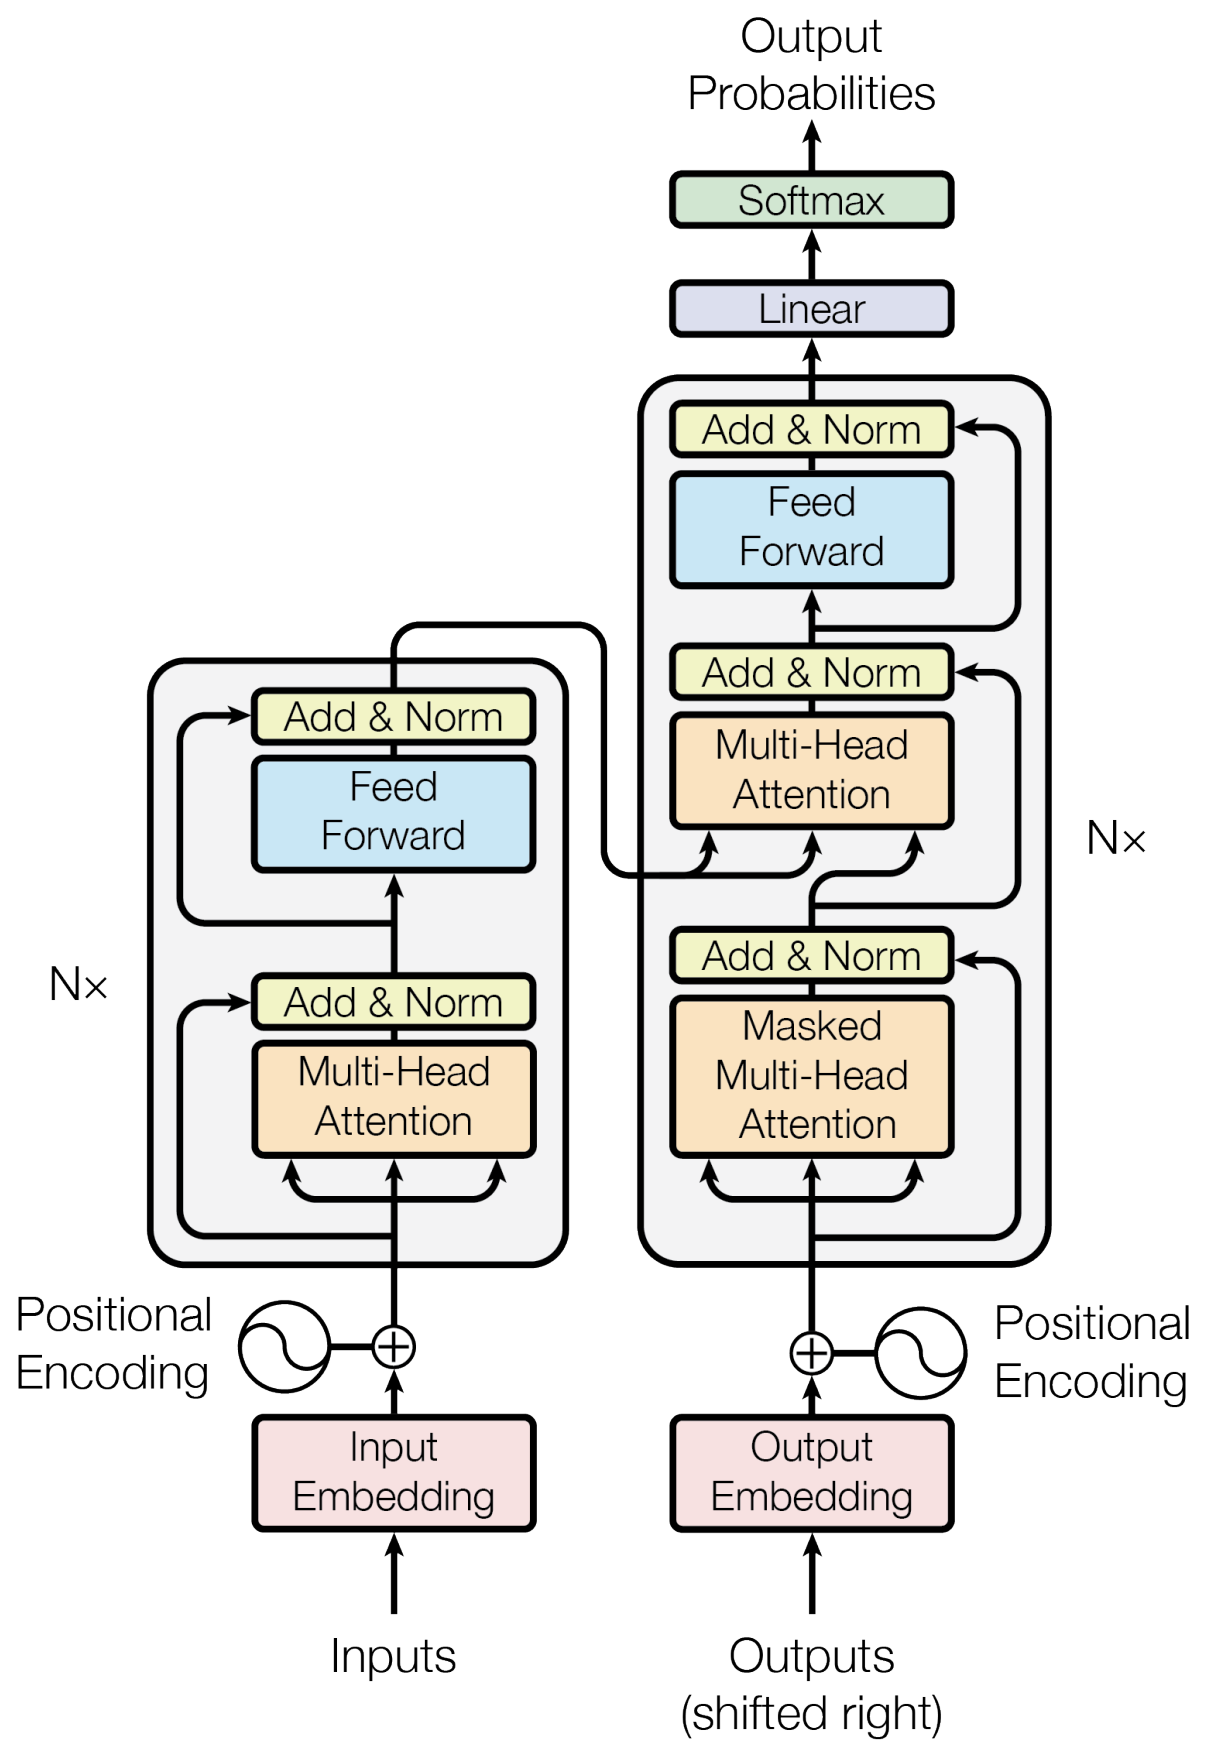
\includegraphics[width=0.4\linewidth]{Figs/transformer.png}
    \caption{The Transformer - model architecture from \citep{DBLP:journals/corr/VaswaniSPUJGKP17}}.
    \label{fig:transformers-arch}
\end{figure}

By looking at the transformer architecture in Figure \ref{fig:transformers-arch} the general model makes use of several blocks throughout the encoder and decoder, like point-wise and fully connected layers. Specifically, both the encoder and the decoder (left and right sides respectively) are composed of a series of overlapping identical layers. The number of these layers, together with their elements, establishes the size of the model and particularly influences the number of parameters it contains. 

Each layer contains several components within it. The first element is the self-attention mechanism, then follows a fully connected feed-forward network. It is important to note that there are residual connections after each sub-layer of the architecture followed by normalization. Specifically, any output from the previous layer is both propagated to the next layer and preserved in its original form in the following way: $\text{LayerNorm}(x + \text{Sublayer}(x))$ where $\text{Sublayer}(x)$ is any type of function from the sublayer itself. As expected, the decoder takes the input from the encoder part of the architecture, implementing the same characteristics observed for the encoder with self-attention, residual connection and Layer Normalization.

An important factor that allows this type of model to outperform any other current neural network architecture is the presence of the self-attention mechanism. Given the input embedding matrix $X$, the self-attention modules multiply it with three weight matrices $W^Q, W^K, W^V$ respectively for queries, keys and values. Those are combined together by the scaled dot-product self-attention as follows:

\begin{equation*}
    \text{Attention} (Q, K, V) = \text{softmax} \left ( \frac{QK^T}{\sqrt{d_k}} \right )
\end{equation*}

where $d_k$ is the shape of the query and keys vectors used as scaling factor for stability purposes. Moreover, this mechanism is repeated in parallel $h$ times, and considering $L$ as the number of total layers stacked together, the total number of attention mechanisms in transformer architecture is $L \times h$. The purpose of using this parallelism, in addition to better computational scalability, is to combine multiple potentially different representations from multiple locations in the text. Given multiple single heads of attention it is possible to achieve:  

\begin{equation*}
    \text{MultiHead} (Q, K, V) = \text{Concat} (\text{head}_1, ..., \text{head}_h) W^O
\end{equation*}

where each head is defined as:

\begin{equation*}
    \text{head}_i = \text{Attention} (QW^{Q}_{i}, KW^{K}_{i}, VW^{V}_{i})
\end{equation*}

As already anticipated, the reasons why this architecture outperforms what has been seen in NLP in the past stem mainly from two factors. 

The first is definitely the scalability of self-attention-based networks, as they are extremely parallelizable and therefore excellent for the computation performed by modern GPUs capable of performing simple computations simultaneously. The advantage of quickly scaling the number of parameters is a feature that will be addressed later in the next chapters along with all the limitations that arise with this feature. 

The second reason lies in the inherent operation of this architecture. In fact, the self-attention mechanism allows for the best representation of the text taken as input, not neglecting the long-range dependencies that were previously difficult to capture, e.g. by recurrent-type networks. The internal attention matrix makes it possible to compare any token in a sentence with any other token regardless of their mutual position and thus their distance. This allowed a representation of the context of the sentence, and thus an understanding of it, that was previously hardly achieved by the state of the art in natural language understanding.


\section {Generative Language Models} 

The language modelling (LM) task is one of the major approaches now used to enable machines to understand natural language. In general, LMs aim to model the generative likelihood of word sequences, so as to predict the probabilities of feature tokens \citep{zhao2023survey}. Formally, let $(y_1, y_2, ..., y_n)$ be tokens in a text corpus (or sentence for simplicity), and $P(y_1, y_2, ..., y_n)$ the probability to see all these tokens following this specific order. By using the chain rule for probability, it is possible to derive the following product:

\begin{equation*}
    P(y_1, y_2, ..., y_n) = P(y_1) \cdot P(y_2 | y_1) \cdot P(y_3 | y_1, y_2) \cdot ... \cdot P(y_n | y_1, ..., y_{n-1}) = \prod_{t = 1}^n P(y_t | y_{<t}) 
\end{equation*}

also defined as a left-to-right language modelling framework, used by most of the generative language models.

Generation is handled differently according to the cases of interest. As anticipated, the next token is taken by considering the probability distribution over the entire vocabulary conditioned on the presence of all previous tokens:

\begin{equation*}
    y_t = \text{argmax}_y \prod_{t=1}^t (P(y | y_{<t - 1}))
\end{equation*}

This technique is defined as greedy search, i.e. selecting the highest probability token at each step. A more widely used approach is called beam search, where multiple candidates (called beams) are considered at each step:

\begin{equation*}
    y_t = \text{argmax}_y \prod_{t=1}^t (P(y^k | y_{<t - 1}))
\end{equation*}

or using log probability:

\begin{equation*}
    y_t = \text{argmax}_y \sum_{t=1}^t \log (P(y^k | y_{<t - 1}))
\end{equation*}

with any $k$-th token in a beam. The advantage of this technique is to select a less constrained generation, and thus an output more similar to human language. Generally, these techniques are combined with parameters such as temperature, top probability (only candidates with a probability above a certain threshold are considered) or top token (a maximum number of tokens to be considered per beam search is imposed).

Pre-trained Language Models, introduced for the first time with ELMo \citep{peters-etal-2018-deep}, were proposed to capture context-aware word representations by pre-training a Bi-LSTM network on a large text corpus and then fine-tuning it according to any specific downstream task. As previously mentioned, after the introduction of Transformers network \citep{DBLP:journals/corr/VaswaniSPUJGKP17} the highly parallelizable and the great learning capabilities of the architecture unlocked new state-of-the-art performance in the area of natural language understanding and representation. BERT \citep{devlin-etal-2019-bert} is one of the first attempts in this regard, achieving never-seen performance on a huge amount of NLP tasks.

Since then, researchers have found that by scaling parameters, better performance could be achieved, both in terms of language representation and generation itself \citep{kaplan2020scaling}. There is a correlation in this regard in terms of the number of parameters and size of datasets that can be used in the pre-training phase, and consequently to the computational power available. These three aspects, directly proportioned, can increase the performance of the models by absolutely guaranteeing their scalability. In addition, the larger the model, the higher its efficiency in terms of data points needed for convergence for further optimization applicable after the pre-training process.


New models, such as 175B-parameters GPT-3 from \citet{brown2020language} (or the most recent GPT-4 from \citet{openai2023gpt4}), 540B-parameters PaLM from \citet{chowdhery2022palm} and LLaMA 2 from \citet{touvron2023llama} showed not only great performances, beating the SOTA for that time, but also enabled new discoveries defined as \textit{emergent-abilities} \citep{wei2022emergent} for solving new and complex task (e.g. reasoning and solving problems expressed in natural language) behaving as few shot learners. A remarkable application of Large-LMs (LLMs) is ChatGPT \footnote{\href{https://openai.com/blog/chatgpt/}{\texttt{openai.com/blog/chatgpt/}}}, where a LLM is adapted to dialogue with the user showing great conversation capabilities with humans.


Experimentally, it has been possible to demonstrate how LLMs are able to achieve different abilities that exceed the random threshold in terms of performance. A non-exhaustive list may include:
\begin{itemize}
    \item \textbf{In-context learning}: the ability of LLMs to learn for examples in the input and provide a solution to a problem just by generating the expected output. This process happens without updating the parameters and further training the model for a specific task. This performance was first observed in GPT-3 \citep{brown2020language} and works well even for strict non-language tasks such as arithmetic tasks.
    \item \textbf{Instruction following} (or tuning): by fine-tuning a LLM with a collection of various NLP tasks (e.g. Question-Answering) it is possible to improve model reasoning performance for seen and unseen tasks described in the form of instructions \citep{NEURIPS2022_b1efde53, sanh2022multitask, wei2022finetuned}.
    \item \textbf{Step-by-step reasoning}: by using chain-of-thought (CoT) prompting strategy \citep{wei2023chainofthought} it is possible to solve complex problems by breaking them down into multiple steps that can be easily solved by the model itself. This approach also allows the model to consider the previous problem step just solved as input, enabling it to reason more effectively during the course of text generation.
\end{itemize}

\subsection{General issues concerning LLMs}

\paragraph{Utilization of LLMs} As mentioned, LLMs, in addition to their excellent performance, bring with them a number of necessary issues to mention. Certainly, there is an issue of computational power to be able to operate these models; the aforementioned ChatGPT (thus all the latest variants of GPTs) or all the other open-source and non-open-source models, with their billions of parameters, require not inconsiderable computational resources. Almost all of the computational load is handled by graphics cards and their memory, which are capable, respectively, of performing the necessary calculations (which usually are parallelizable matrix multiplications) and keeping a large amount of associated parameters in memory. Despite the progress of the semiconductor engineering industry, it is still very difficult to be able to pre-train (or even infer) without having computational clusters costing millions. 

To provide a concrete example of the pre-training of a LLM, BLOOM \citep{workshop2023bloom} is a 176-billion-parameter model trained by BigScience, a cooperative organization among several institutions and companies in the research and AI field. The training process has been made completely open-source, giving the ability to look at both the techniques and the amount of time and resources spent training the model. Specifically, the pre-training process employed a total of 384 Nvidia A100 80GB GPUs distributed across 48 nodes (416 of the same GPUs over 52 nodes if we include the backup system), each equipped with top-tier CPUs and half a terabyte of RAM. The dataset includes a total of 46 different languages for an occupied space of nearly 2TB. A single training epoch (i.e., a single pass over the entire dataset) took 3.5 months H24 to complete, with several backup infrastructures for failures due to the hardware employed. The total cost is estimated to be between $2-5$\$ millions just and exclusively for computational resources and cloud computing, thus excluding costs related to training set-up time and all personnel involved.

For this reason, the vast majority of these models are the exclusive preserve of the largest technology companies, the only ones who can currently afford this kind of cost. However, new solutions are constantly emerging in research that allows these models to be used on \textit{prosumer hardware} as well, i.e. hardware that is certainly high in cost but more accessible to the researcher market. This will be addressed in a later chapter (\ref{chapter:model-scale}) regarding the research project under discussion.

Other issues, which can be directly linked to the size of the models, include their environmental impact in terms of resources used (i.e., energy and materials used in their realization and deployment process, \citep{strubell-etal-2019-energy}), as well as their democratization in terms of access to people from all over the world, both in terms of technological and linguistic availability.

\paragraph{Data used for pre-training a LLM} The importance of data, especially in the presence of billions of parameters, is fundamental to pre-train an effective LLM \citep{hoffmann2022training}. To develop a capable LLM a large amount of natural language corpus from various data sources is needed. Usually, existing LLMs mainly leverage a mixture of diverse public textual datasets. Most of the data comes from web pages, books and conversational text helping the model to generalize better and grasp patterns from natural language in various styles and scenarios. In some cases pre-train corpus supplements the original data with scientific corpus, code, and task-dependent data \citep{chowdhery2022palm, zhang2022opt}. Especially in data collected from the Web, control is often applied automatically by different types of filters, but these do not always succeed in capturing only quality text. In addition to popular vetted sources, such as Wikipedia, low-quality text, spam or content from questionable sites are also included in datasets, eventually expanding the trainset with fake news, toxic content or even illegal or immoral information. Another problematic source is conversational text, which, on the one side, improves performance in tasks such as question-answering or factual knowledge, but on the other side includes features that can be typical of Internet dialogues. These issues, especially common to social networks, include the most varied and uncontrolled conversations on topics that are often unethical or even borderline legal. Other issues are often related to privacy or the authority that holds rights to specific data that end up being used as training corpus without any \textit{a priori} permission.

All of this results in a number of issues being passed directly from the data to the model being trained. Indeed, in the large amount of data collected, there are issues that mirror what can be observed in human society (or, at least, the internet society). This type of problem opens up a wealth of questions, scientific and otherwise, concerning precisely the safety and reliability of the models themselves. Selecting these data is by no means an easy task, considering the scale of the problem, and often they are used blindly trying to correct in the post-training phase most of the issues of the models.


\section{Towards helpful, honest, and harmless LLMs}

As anticipated, the size of the data used in the pre-training steps for LLMs succeeds in getting excellent results in the vast majority of benchmarks currently in the literature. However, using such a large amount of data brings with it a number of more or less obvious implications regarding the quality of the data and the content they carry. Being taken from the Internet, in fact, encoded stereotypes and denigrations aimed at minority groups by gender, race, ethnicity, social status and so on are easily identifiable in the trained models \citep{10.1145/3442188.3445922a}. It is also important to emphasize how the size of the models, which we have observed as increasing in recent years, does not bring with it a more accurate representation of social diversity, but rather, precisely because of the data collection mechanisms, often increases the problems previously partially listed.

Given the impossibility of perfectly controlling the data collected in the pre-training phase (consider, e.g., the presence of unintended bias \citep{10.1145/3278721.3278729}, which is difficult to identify especially in large corpora), an attempt was made to develop techniques that could ensure, after the pre-training process, an alignment of the same with what are the human values and considered most correct by today's society.

In general, through the use of these techniques, the aim is to balance three macro-values (or model's characteristics) defined as \textit{alignment criteria} \citep{NEURIPS2022_b1efde53, askell2021general}: 
\begin{itemize}
    \item \textit{Helpfulness}: A model should help, assisting the user with information that is relevant and pertinent. It should therefore follow what is the user's intention, providing concrete help.
    \item \textit{Honesty}: The model should provide the user with information that is real and not produced by recombining its parameters. In this sense, a degree of uncertainty indicating the dissemination of incorrect or misleading factual information should also be considered.
    \item \textit{Harmless}: the model should be as least offensive and discriminatory as possible. It should also not provide information that impinges on the freedoms of others or instructions on how to prosecute acts that go against the jurisdiction in which it operates.
\end{itemize}

The \textit{honesty} aspect, of all three, is probably the most measurable, being composed mainly of factual information that can be verified with standard metrics already found in the literature.
Different argument, however, concerns the \textit{helpfulness} and \textit{harmlessness} criteria, which can sometimes conflict with each other in some borderline cases. Consider, for example, the case where a model is asked to discuss a "hot" topic, that is, one that is very close to speech that is generally classified as hate speech and discrimination against minorities. It is very likely that the model will refuse to respond in order to align with the \textit{harmlessness} criterion, or will respond with something toxic in order to help the user by aligning with the helpfulness criterion. Dealing with these edge cases is what the literature pushes for, trying to find the best possible compromise between two fundamental aspects to achieve a useful and safe model.



\subsection{Latest development on Instruction Tuning and RLHF}
\label{section:technical-Istruct-RLHF}

Among the most widely used technical approaches in the literature for aligning models to human intent in post-training is certainly the use of Instruction Tuning \citep{NEURIPS2022_b1efde53, min-etal-2022-metaicl, NEURIPS2020_1f89885d} and Reinforcement Learning from Human Feedback / AI Feedback (RLHF / RLAIF) \citep{christiano2023deep, gao2022scaling}.

\paragraph{Instruction tuning} LLMs, following their pre-training phase, do not perfectly follow human behaviour but continue to produce output based on previous tokens without structuring the information or following user requests. For this reason, Instruction Tuning fine-tunes a model to predict a certain response given a prompt but produces a well-structured output based on the instruction received as input in the prompt. Generally, these instructions are based on common NLP tasks, allowing the models to generalize better to unseen tasks. This technique also improves the model generalization capabilities making them zero-shot learners \citep{wei2022finetuned, sanh2022multitask}, i.e. the ability of the model to learn at test time, learning just by looking at the prompt without any update on parameters required. This is possible given the ability of fine-tuning to still preserve the original weights of the model and thus its ability to reason about given tasks. These prompt engineering techniques allow these reasoning capabilities to be better exploited, making the models also useful as end-user assistants. Collection of instruction, like FLAN in \citet{wei2022finetuned}, contains multiple NLP-task datasets aggregated under the same template, including tasks such as Natural Language Inference, sentiment, commonsense, question-answering, reading compensation, summarization, translation and many others.

From a technical point of view, the instruction-tuning procedure fine-tunes the model on the same task used during pre-training, i.e. next-token prediction. By doing so, the model's parameters are optimised towards generations that take the input into account and reason on it, generating responses that answer or solve the problem initially posed. In the larger models (LLMs), this leads to excellent generalisation capability even on tasks never seen, leading to the hypothesis that the fine-tuning process allows for accurate understanding in the submitted task rather than generation based on what was seen in the pre-training. More striking applications in this sense can be found in models that are optimised to behave as chat-bots\footnote{Examples in this sense may be OpenAI's \href{https://chat.openai.com/}{\texttt{ChatGPT}}, Google's \href{https://bard.google.com/}{\texttt{Bard}} and many others, also domain-specific.}, i.e. they have the ability to answer questions and engage in conversation on a given topic based on the context preceding a given generation.

Importantly, this process pushes the model to be as helpful as possible to the user (\textit{helpfulness criteria}). Also, this process then inevitably leads to the possibility of attacks that elicit unintended behaviour, being able to effectively control toxic conduct, or models being used for borderline purposes \citep{shu2023exploitability}. The low sample complexity and requirements of instruction tuning enable the possibility to alter the behaviours of LLMs with small training efforts, usually called poison attacks. Indeed, it is possible to train models by following specific behavioural patterns that an organization want to maintain by using modified instructions. Models trained in this way will carry with them these examples and produce "poisoned" outputs even in the presence of totally legitimate prompts.




\paragraph{Reinforcement Learning from Human Feedback} The emergence of approaches based on reinforcement mechanisms, instead of the previously fine-tuned approaches on specific tasks, arose mainly to adapt models to tasks or behaviours that are by their nature difficult-to-specify \citep{ziegler2020finetuning, Bai2022TrainingAH}. These techniques make it possible to go beyond training data, better generalising the different tasks and behaviours of the models that most closely align with human preferences. 

From a technical point of view, the high-level process collects human feedback on a series of generations, usually from an already instructed model. Note that feedback can also come from a predictive classifier model that provides a metric on how well a generation may be aligned with human preference \citep{lee2023rlaif}. This metric is incorporated into the model's reward system which is then optimised through the use of a policy, usually PPO from \citet{schulman2017proximal}. The process, briefly illustrated in figure \ref{fig:rlhf-procedure} starts with the initial base model $\pi_{\theta}$ where $\theta$ are its pre-trained parameters, generating a distribution of examples over a pre-defined dataset. The following step is to collect the human feedback (or AI feedback) $r_H$ over each example. Let a function $f$ map each example $x_i$ to its corresponding feedback (or reward $r_H$) given by the user $H$, and $\epsilon$ as a random noise the final feedback $y_i$ will be:

\begin{equation*}
    y_i = f(H, x_i, \epsilon_i)
\end{equation*}

By having all the feedback given by the human $H$ it is possible to fit a reward model $\hat{r}_{\phi}$ to approximate $H$ evaluation as closely as possible. With a dataset of examples $\mathcal{D} = {(x_i, y_i)_{i = 0,...,n}}$ the parameters $\phi$ are trained minimizing the following function:

\begin{equation*}
    \mathcal{L}(\mathcal{D}, \phi) = \sum_{i = 0}^{n} l(\hat{r}_{\phi}(x_i), y_i) + \lambda_r(\phi)
\end{equation*}

with $\lambda_r$ being any type of regularizer. The final parameters of the model are obtained through the minimization of the aforementioned loss function $\mathcal{L}$. New parameters at each step are obtained as follows:

\begin{equation*}
    \mathcal{R}(\theta_{\text{ new}}) = \mathbb{E}_{x \sim \pi_{\theta_{\text{ new}}}} 
        [\hat{r}_{\phi}(x) + \lambda_p (\theta, \theta_{\text{new}}, x) ] 
\end{equation*}

\begin{figure}
    \centering
    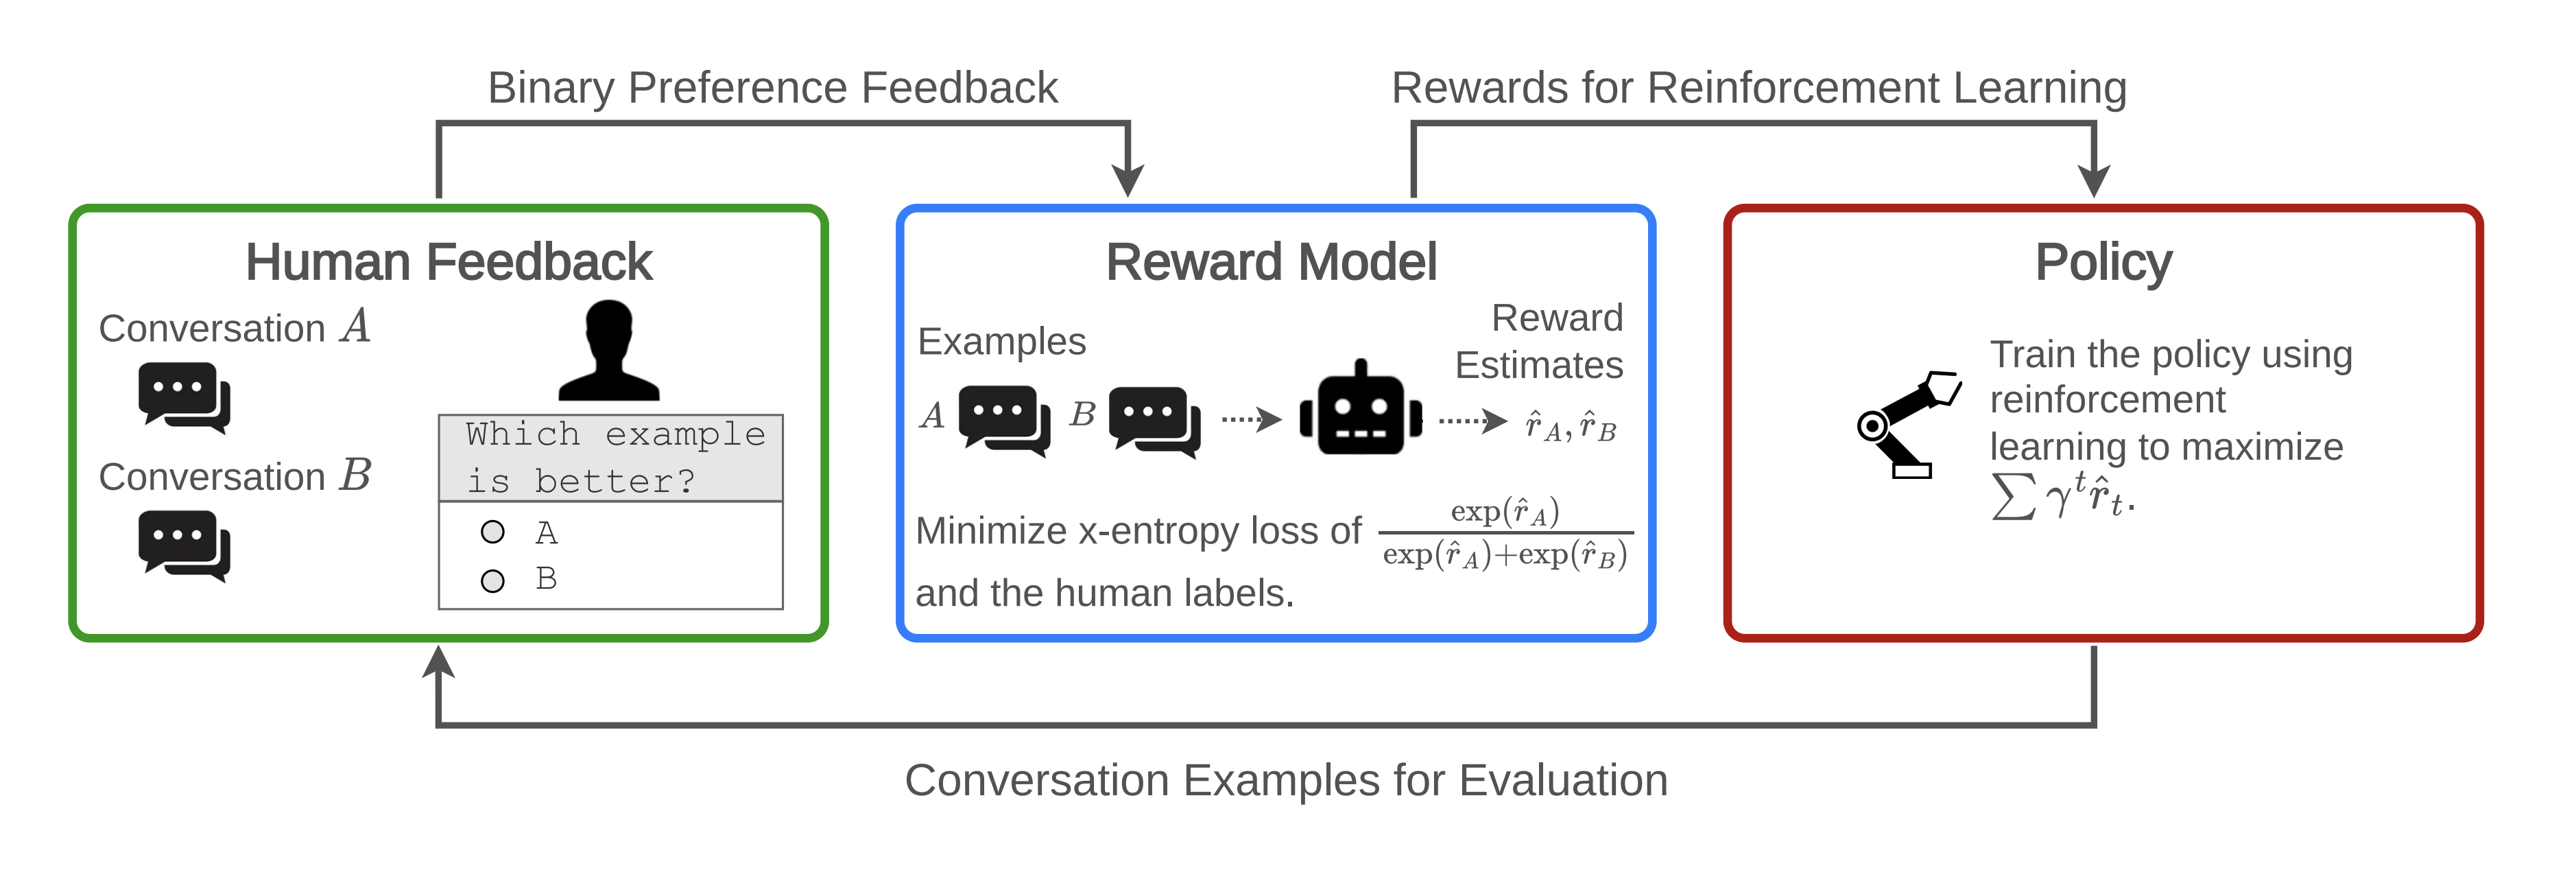
\includegraphics[width=0.99\linewidth]{Figs/rlhf-procedure.png}
    \caption{Illustrated RLHF procedure with a binary feedback provided by the human. From \citet{casper2023open}.}
    \label{fig:rlhf-procedure}
\end{figure}


Generally, $\lambda_p$ is some divergence-based regularizer. The most adopted solution is based on the KL-divergence:

\begin{equation*}
    D_{KL} (P || Q) = \sum_{x \in X} P(x) \log{ \left ( \frac{P(x)}{Q(x)} \right )} = - \sum_{x \in X} P(x) \log{ \left ( \frac{Q(x)}{P(x)} \right )} , 
\end{equation*}

namely a measure of how one probability distribution $P(\theta_{\text{ new}})$ is different from a second, reference probability distribution $Q(\theta)$ with $\theta_{\text{ new}}$ and $\theta$ being respectively the model updated by the PPO procedure and the reference model whose parameters are kept frozen. This measure of statistical distance is employed in this project to prevent model parameters from diverging from the original.

As for the PPO optimization procedure, introduced in 2017 by OpenAI \citep{schulman2017proximal}, appears to be the best balance between optimization performance and ease of implementation. The Proximal Policy Optimization implementation is very close to the original policy gradient but through small changes the algorithm is optimized to outperform the vanilla one in most of the cases.

As previously introduced, given a set of tunable parameters $\theta$, the aim is to update in the direction that yields higher rewards as possible. The policy $\phi_\theta (a | s)$ is defined as stochastic, i.e. the parameters are the only ones that dictate the probability of an action $a$ directly influencing the trajectory $\tau$ defined as a sequence of pairs of states and action $s_1, a_1, ..., s_n, a_n$.

The objective function that PPO aim to optimize is defined as follows:

\begin{equation*}
    J (\theta) = E_{\tau \sim \pi_\theta} R(\tau) = \sum_\tau P(\tau; \theta) R(\tau)
\end{equation*}

By using the stochastic policy, the goal is to sample various actions, recording the corresponding probability and the differences in rewards. Applied to language model generation this means that the model generates a response to the given prompt and then is optimized at each step (if the batch size is equal to 1 sample per time) according to the given reward. To determine the update direction in which the model is optimized, policy gradient methods rely on gradients $\nabla_\theta$, which corresponds to a vector of partial derivatives for the target function (or model). The update is therefore performed according to the function:

\begin{equation*}
    \theta \leftarrow \theta + \alpha \nabla_\theta J(\theta)
\end{equation*}

with $J(\theta)$ embedding the reward function and $\alpha$ being the learning rate. Finding a good learning rate turns out to be a non-trivial problem. In fact, optimization processes of this type tend to over-weight the optimization step by leading the updated model to diverge. For this reason, the proximal policy optimization process, restricts the range within which the policy can be updated. This is performed by a small change to the objective function by clipping the steps according to different cases. The new objective function is defined as follow:

\begin{equation*}
    L^{CLIP}_{\pi_\theta} (\pi_{\theta_k}) = \mathbb{E}_{\tau \sim \pi_\theta} \left[ \sum^T_{t = 0} \left[ \min \left( \rho_t (\pi_\theta, \pi_{\theta_k}) A^{\pi_{\theta_k}}_t , \text{clip}(\rho_t (\pi_\theta, \pi_{\theta_k}), 1 - \epsilon, 1 + \epsilon) A_t^{\pi_{\theta_k}} \right) \right] \right]
\end{equation*}

with the importance sampling ratio $\rho_t$ as a value given by the ratio between the original model $\pi_\theta$ and the updated model $\pi_{\theta_k}$:

\begin{equation*}
    \rho_t (\theta) = \frac{\pi_\theta (a_t | s_t)}{\pi_{\theta_k} (a_t | s_t)} 
\end{equation*}

By analyzing the new objective function, the minimum among all the terms listed (in addition to the clip of some elements) is calculated for conservative issues in terms of optimization, in other words to avoid optimizing strongly toward a direction (new state $s_t$) that may lead to worse future actions ($a_t$). Instead, the $1 - \epsilon$ and $1 + \epsilon$ terms do not depend on the model's parameters $\theta$ but are imposed as boundaries of the region within which the model can move.

In spite of the lack of strong theoretical and mathematical evidence on the convergence of this algorithm \citep{schulman2017trust}, it has been multiply demonstrated that on the empirical level this procedure is generally the fastest and most effective in terms of convergence in the optimization process for reinforcement learning.

Moreover, the structure of the PPO algorithm imposes greater use of the available graphical memory. This happens because two exact copies of the same model in their initial state must be kept in memory, and then only one of these two is updated according to the optimization process. The original version, however, must be held in memory until the end of training. This generally leads to computational complications, but these can be mitigated as explained in later chapters.



\section{Interpretability of Language Models}

Generating human-understandable explanations for the behaviour of AI systems is currently an unsolved problem. Due to their immense complexity, LLMs are generally considered black-box models and this brings with it a number of problems related to the use of LLMs in risky environments where safety, reliability and accountability are necessary features \citep{rudin2019stop}. Although metrics are currently used to measure the effectiveness of models under a large number of different tasks, they still fail to capture all the probable cases of failure that one might have or, better still, fail to explain how a given model makes a decision and what the reasons for it are. The aim of the current research project is to investigate methods of interpretability defined as \textit{post-hoc}, i.e. methods that provide an interpretation of models already trained according to the procedures seen above and that are as agnostic as possible to the model itself.

There are different approaches to interpretability:
\begin{itemize}
    \item Gradient-based: these approaches try to capture the gradient w.r.t. the input by measuring the change of output given an $\epsilon$-change to each input feature \citep{li-etal-2016-visualizing}. This method is defined as functionally grounded but does not always guarantee a trustworthy explanation for non-linear models since the explanation relates to a first-order Taylor approximation.
    \item Perturbation-based: these explanation methods are based on nearby observations $\hat{x}$ of the input $x$. With LIME the model estimates $p(c|\hat{x})$ to fit a logistic regression. The parameters of the logistic regression represent the importance measure \citep{ribeiro-etal-2016-trust}.
    \item Internals-based: For transformer-based models, the attention could provide a good explanation of what the model looks and, consequentially, give importance in order to generate a specific output. By doing so it is possible to look at all the internal layers and parameters to explain the model's behaviour. It is not clear if attention could be considered as an interoperability technique since it does not always provide a good or meaningful output explanation \citep{bibal-etal-2022-attention}.
\end{itemize}

By definition, interpretability techniques aim at explaining a model output to humans \citep{MILLER20191} and, consequentially, they are developed to provide a qualitative explanation. This characteristic leads to difficulties in comparing or quantitatively evaluating any method proposed. Generally, this problem is tackled by checking the meaning of the results found at the human level, and then proceeding with more precise quantitative evaluations. However, there are as yet no standards or guidelines in this regard, leaving the choices to the discretion of the researcher.

Progress in explainability and interpretability could help verify hypotheses about how models make decisions \citep{geiger2023causal} and help in verifying the decision process of the model. A model or process that can be explained would give greater confidence and trust in its decision-making processes, ensuring more than the use of metrics on standard benchmarks the ability not to fail under certain circumstances \citep{jacovi2021formalizing}. Furthermore, an analysis of a model that includes interpretability as a fundamental step could better explain its vulnerabilities. Specifically, looking at model red-teaming attempts \citep{ziegler2022adversarial}, in the case of identifying adversarial inputs it would be possible to generalise the reasons why a given model is prone to fail in that circumstance \citep{rastogi2023supporting, räuker2023transparent}.

Various interpretability techniques could be employed to improve specific aspects of the models, acting on their internal behaviour and improving, for instance, their truthfulness \citep{li2023inferencetime}, changing the factual knowledge they contain \citep{meng2023locating, hernandez2023inspecting} or directly steering their behaviour for certain aspects.

% How interpretability could help:
% Interesting "Interpretability and model editing" paragraph from https://arxiv.org/pdf/2307.15217.pdf

%!TEX root = ../thesis.tex
%*******************************************************************************
%****************************** Third Chapter **********************************
%*******************************************************************************
\chapter{Approach and Experimental Setup}

This chapter will present the motivations and approaches that led to the research questions posed during the project work. The steps followed to achieve the obtained results during the research work will then be addressed.


The entire code base enabled the building of a toolkit capable of assisting in the post-training of the models for the purposes of detoxification, the measurement of the level of toxicity of the models, and finally, the exploration of the final models through automated interpretability techniques as proposed in the next chapters\footnote{GitHub repository available at: \href{https://github.com/DanielSc4/RewardLM}{RewardLM, via GitHub}}.

\section{Line of Research}

As already seen, during the exploration of the state of the art in chapter \ref{chapter:SOTA}, a number of issues related to modern Language Models arise as important questions on which more effective and efficient solutions need to be sought. Moreover, their characteristic of being difficult to explain, makes the process more difficult and challenging from a scientific point of view, having to bring improvements not only in terms of performance but also to think further about the possibility of effectively understanding the reasons why certain mechanisms work as intended.

To this end, various post-training techniques are usually applied but it is not yet entirely clear how these contribute to the improvement of the model itself. While it is necessary to achieve better performance, it is also important to ensure as far as possible that the observed results are persistent over a large number of possible inputs. It is therefore of paramount importance to be able to generalise these aspects, no longer by looking at "standard" metrics, but by being able to grasp why models assume a certain behaviour. As seen, model interpretability points precisely in this direction and can be considered a useful tool for this purpose.

The aim of this project is therefore precisely to use generative models that represent the state of the art in their class and investigate how the most widely used detoxification processes (fine-tuning and RLHF) make them safer while retaining their ability to help the end user who uses them. With these objectives in mind, it is then necessary to investigate how the model has been modified internally by these processes. This step is of fundamental importance in order to be able to observe and understand the strengths and weaknesses of each technique employed, as well as provide a useful aid in identifying any issues still to be resolved in current Language Models.

The next sections will explain in detail how this line was applied in practice, from the choice of models and data to be used in the experiments to the technological adaptations used for the setup that enabled the required results to be obtained.


\section{Employed models} 
\label{chapter:model-selection}

As a first step, currently state-of-the-art models are chosen for performance based on standard metrics measured directly from the leaderboard of HuggingFace \footnote{Leaderboard available at the following link: \href{https://huggingface.co/spaces/HuggingFaceH4/open_llm_leaderboard}{Open LLM LeaderBoard, via HuggingFace}}, a standard library for managing the latest Language Models.

During the selection of models, special attention was placed on their architecture, with a particular preference toward decoder-only models for their setup simplicity during the following experiments. Further consideration was given to the performance factor as a metric to evaluate the initial quality of the model based on the number of parameters kept under 7 billion for computational reasons. The choice of models, therefore, fell on the RedPajama family \citep{together2023redpajama}, specifically the specialized version for chatbot-style behaviour \footnote{Model id on HuggingFace: \href{https://huggingface.co/togethercomputer/RedPajama-INCITE-Chat-3B-v1}{ \texttt{togethercomputer/RedPajama-INCITE-Chat-3B-v1}}} (i.e., pre-trained version, instruction-tuning and RLHF) and the Falcon family \citep{falcon}, again in its instructed version\footnote{Model id on HuggingFace: \href{https://huggingface.co/tiiuae/falcon-7b-instruct}{ \texttt{tiiuae/falcon-7b-instruct}}}. In the first case, with RedPajama, the total number of trainable parameters is 3 billion, while in the latter case, the total corresponds to 7 billion. It can be seen that both models have already been pre-trained and have already gone through an open-source detoxification process (both instruction tuning and RLHF). This means that the datasets on which the training processes were carried out are already available to the open-source community and are in continuous evolution and improvement by the community itself. These optimization processes already addressed by the models have sensibly lowered their starting toxicity but we aim to still be able to lower it even more with different \textit{ad-hoc} techniques later explained.


As far as the reward module for the algorithm based on reinforcement learning, a RoBERTa class model \citep{vidgen-etal-2021-learning}, fine-tuned for the toxicity detection task\footnote{Model id on HuggingFace: \href{https://huggingface.co/facebook/roberta-hate-speech-dynabench-r4-target}{\texttt{facebook/roberta-hate-speech-dynabench}}} was chosen because of its known performance on different types of benchmarks employed in the literature \citep{vidgen-etal-2021-learning}.


\section {Data: Counter-narrative}
\label{chapter:counter-narrative}

One of the main goals of this research work, as anticipated in the introduction of this thesis, is to give models the opportunity to be able to express themselves beyond the barriers commonly imposed for dialects considered toxic. As noted in \citet{röttger2023xstest} often the limitations imposed in the post-training phase of models turn out to be excessive, resulting in a response that denies any further conversation following a specific prompt that may be toxic or misinterpreted as toxic. Instead, during the post-training performed here, we want to explore more the capacity of the models themselves in terms of argumentation, leaving the generation free even in the presence of prompts considered toxic. This aspect is generally carried through guardrails imposed on the models, leading them to produce output following hidden guidelines. However, these mechanisms are not resilient to attacks through prompts that still manage to overcome these impositions. What is hoped to achieve is thus a model that can offer a counter-narrative to toxic prompts, giving them importance and providing at the same time a counter-response that highlights fallacies or otherwise challenges the original claim.

These choices lead to improving the helpfulness of aligned Language Models by encouraging the generation of ``[...] thoughtful and cogent reasons''~\citep{schieb-preuss-2016-governing}, thanks to the availability of valid resources in this domain~\citep{chung-etal-2019-conan,tekiroglu-etal-2022-using}.

To achieve this, the choice of training data, therefore, turns out to be of paramount importance. From the work of \citet{bonaldi-etal-2022-human}, is presented a dataset that provides a set of dialogues, between a user and a counter-user that meet the criteria previously described. The prompts written by the user are considered toxic while the response given by the counter-user tries to explain and establish a polite dialogue about the topic that the user initially proposed. Specifically, the dataset contains not only pairs of prompt and response but multiple pairs of them simulating a proper dialogue. An example of dialogue from the \texttt{DIALOCONAN} is provided in Table \ref{tab:example-dialoconan}


% If you use beamer only pass "xcolor=table" option, i.e. \documentclass[xcolor=table]{beamer}
\begin{table}
\small
\centering
\begin{tabular}{ll}
\toprule
User & Message \\ 
\midrule

{\color[HTML]{CB0000} Hater} & \begin{tabular}[c]{@{}l}Women getting into the labour market has caused \\ the downfall of Western civilisation, they should be \\ at home raising children. Abandoning traditional roles \\ is the ruin of society.\end{tabular} \\ 
\cmidrule(lr){2-2} 
{\color[HTML]{00009B} Counter-narrative} & \begin{tabular}[c]{@{}l}I'd disagree, women should be able to choose \\ what they do, but also even if some women did want \\ to stay at home, many don't have a choice anymore! \\ It's impossible to support a family on 1 wage now.\end{tabular} \\ \cmidrule(lr){2-2} 
{\color[HTML]{CB0000} Hater} & \begin{tabular}[c]{@{}l}Oh really? It didn't used to be impossible, \\ it used to be the norm, what's changed?\end{tabular} \\ 
\cmidrule(lr){2-2} 
{\color[HTML]{00009B} Counter-narrative} & \begin{tabular}[c]{@{}l}The cost of living has increased rapidly whilst wages \\ have stagnated over the last few decades. \\ This means that whilst 1 full time wage used to support \\ a family, now with proportionately higher prices \\ for things like food and housing, this isn't possible.\end{tabular} \\ 
\bottomrule

\end{tabular}
\caption{Example from the \texttt{DIALOCONAN} dataset. Dialogue involves a hater and a control narrative written by an expert user.}
\label{tab:example-dialoconan}
\end{table}


Given the size of the models, and therefore, the large amount of data needed to train them, it was decided to perform a split of the dataset that would fully exploit the composition of the dialogues themselves. Specifically, all pairs in the dataset are employed while maintaining the previous context in case there are previously given answers. This made it possible to obtain a dataset with $8312$ conversation pair, useful for subsequent post-training phases.

Looking at how this data will be used by the techniques explained in the previous section \ref{section:technical-Istruct-RLHF}, it is expected that fine-tuning will fully capture the counter-narrative characteristics contained in the dataset. The fine-tuning process of the models is based on the task of next token prediction \citep{DBLP:journals/corr/VaswaniSPUJGKP17} where the parameters of the model are shifted according to the prediction of the next token based on all previously seen tokens \citep{solaiman-christy-2021-palms,zhou-etal-2023-lima}. This technique is probably the best to "steer" a model towards a precise generation dependent on the distribution of the training data.

A different approach is taken with reinforcement learning, where, despite the presence of the data, no constraint is placed on the generation of the individual tokens and the model is optimised by following only the reward provided by the model or the training system in which it is inserted \citep{schulman2017proximal}. The generation of counter-narratives is therefore not an aspect we expect to see other than a general reduction in the toxicity of the model both on the test dataset, which respects the initial distribution of \texttt{DIALOCONAN}, and in terms of general toxicity later explained in more detail.





\section {Addressing model scale}
\label{chapter:model-scale}

As anticipated, with the growth in terms of model parameters (surpassing even a hundred billion as in \citet{openai-2023-gpt4}), more and more computational resources are required not only for training but also for inference on these models. 

By looking at the estimations provided by the Model Memory Calculator \footnote{\href{https://huggingface.co/spaces/hf-accelerate/model-memory-usage}{Model Memory Calculator}} is it possible to estimate how much vRAM is needed for both inference and training using an Adam class optimizer from \citet{Kingma2014AdamAM}. The amount of vRAM required for Falcon (having 7 billion of total trainable parameters) to train using \texttt{32-bit} precision would be around 107.54 GB, more than what is made available by the popular Nvidia A100 (or H100), currently the highest performing GPUs on the market dedicated to scientific computation with 40GB and 80GB depending on the specific version. These issues have long made it difficult for researchers to carry out experiments with this type of model, limiting their access to more powerful models that could then provide better results.


\subsection{8-bit approximation}

Most of the parameters ($\sim 95\%$) of models based on the transformer-like architecture \citep{DBLP:journals/corr/VaswaniSPUJGKP17},  are concentrated on the feed-forward layers and the projections of the attention matrices in the self-attention module; the self-attention mechanism, on the contrary, does not contain any parameters but consists only of matrix transformations that allow measuring the importance of different tokens for the context representation. One known way to decrease the space occupied by these matrices is to use quantization techniques to represent the parameters in a less precise format than the standard \texttt{32-bit} format, trying to keep performance as close to the original model as possible.
In most cases, the best approach was to halve the precision of the \texttt{16-bit} matrices or do a mix between full precision (\texttt{32-bit}) and half-precision (\texttt{16-bit}).

Despite these techniques, however, given the size of the latest state-of-the-art models, the \texttt{16-bit} representation is still computationally expensive. For this reason, an \texttt{8-bit} quantization technique is introduced in \citet{dettmers2022llmint8} that can decrease the computational load in terms of resources for inferring models with billions of parameters while effectively managing to maintain the performance seen relative to the full-precision version. The same technique later led to the use of an even smaller \texttt{4-bit} representation in \citet{dettmers2023case}, further reducing the load on resources from the models by almost half.

Specifically, the particular importance regarding the presence of outliers in the model parameters is addressed where, in the case of approximation due to the direct quantization from \texttt{16} to \texttt{8/4-bits}, considerable performance degradation was observed. Specifically, the scaling consists of a standard Absmax quantization (see \ref{eq:absmax-quant}) from a half-precision tensor and a zero-point quantization for asymmetric distributions (e.g. from ReLU function output) in order to use the full $[-127, 127]$ range available.

\textbf{\textit{Absmax quantization}} in \ref{eq:absmax-quant} scales inputs to the \texttt{8-bit} range. $s_{x_{f16}}$ is $127$ divided by the absolute maximum of the entire tensor which is equivalent to dividing by the infinity norm.

\begin{equation}
    X_{i 8} = \biggl \lceil \frac{127 \cdot X_{f16}}{\max_{ij}{(|{X_{f16}}_{i,j} |)}}  \biggr \rfloor = 
\biggl \lceil \frac{127}{||X_{f16}||_{\infty}} \cdot X_{f16} \biggr \rfloor = 
\lceil {s_x}_{f16} X_{f_16} \rfloor
\label{eq:absmax-quant}
\end{equation}

\textbf{\textit{Zeropoint quantization}} in \ref{eq:zeropoint-quant} shifts the input distribution into the \texttt{8-bit} range by scaling the normalized dynamic range $nd_x$ and shifting by the zeropoint $zp_x$. This affine transformation reduces the quantization error for asymmetric distributions.

\begin{equation}
\begin{gathered}
nd_{x_{f16}} = \frac{2 \cdot 127}{\max_{ij} ( X^{ij}_{f16} ) - \min_{ij} (X^{ij}_{f16})} \\ 
zp_{x_{i16}} = \lfloor X_{f16} \cdot \min_{ij} (X^{ij}_{f16}) \rceil \\
X_{i8} = \lfloor nd_{x_{f16}} X_{f16} \rceil
\end{gathered}
\label{eq:zeropoint-quant}
\end{equation}

In addition, with the aim of preserving outliers between rows and columns of the matrix of interest, a \textit{vector-wise quantization} is proposed and, in some cases the presence of \textit{mixed precision} between \texttt{8} and \texttt{16-bit} where necessary. Experimentally, a net reduction of just over half in terms of memory occupied has been observed even for transformer models with billions of parameters consequently leading to run times close to twice the speed if compared to the original model.



\subsection{Parameter-Efficient Fine-Tuning (PEFT) and LoRA}
\label{chapter:LORA}

% look at https://towardsdatascience.com/dive-into-lora-adapters-38f4da488ede could be useful

As seen, it has been possible to use prosumer hardware to employ large dimensional models through quantization techniques. The main problem, however, is the training procedure, which is not effective when the bit range is as low as \texttt{8} or \texttt{16-bit}. For this reason, over the past few years, as the average model size grew beyond multiple billion parameters, several techniques were proposed to train such large models even with limited computational resources. Chief among them is to fine-tune only a small subset of original trainable parameters starting from an already pre-trained model. The main problem with these techniques, however, is inference latency \citep{houlsby2019parameterefficient} or reduction in usable sequence length \citep{lester2021power, hambardzumyan2021warp}; in other words, a major trade-off between efficiency and the quality of the model itself.

With the introduction of LoRA in \citet{hu2021lora} pre-trained models can be freezed and thus kept in any precision format while training adapters (called LoRA modules in this specific case) leading to a reduction of storage and computational power requirements. Also, a new and more efficient training procedure is also adopted for adaptive optimizers not needing to maintain the states for most parameters.


The idea behind Low-Rank adapters to be used with original frozen pre-trained weights is to train adapters that can be stored even without the original model, thus lighting the process of deployment an entire model for every single task. By adopting a smaller-sized set of parameters $\theta$ (much lower than the number of parameters from the original pre-trained model) the task of optimizing the conditional language modelling objective becomes:

\begin{equation*}
\centering
    \max_{\theta} \sum_{(x, y) \in Z} \sum_{t = 1}^{|y|} \log \left( p_{\Phi + \Delta \Phi(\theta)} (y_t | x, y_{< t}) \right)
\end{equation*}

where the model is initialized to pre-trained weights $\theta$ and updated to $\phi + \Delta \phi$ at any give time.

Specifically, the paper introducing Low-Ranks adapters focus its attention on proposing low-rank representation to encode $\Delta \Phi$ in both compute and memory efficient way, allowing for a subset of parameters low as small as $0.01 \%$ of the original pre-trained weights $|\Phi|$. Inspired by \citet{aghajanyan-etal-2021-intrinsic}, pre-trained language models have a low "intrinsic dimension" that can still learn despite the smaller subspace, so the learning process that updates the matrix $W_0 \in \mathbb{R}^{d \times k}$ can be represented by a low-rank decomposition $W_0 + \Delta W = W_0 = BA$; this yield to a final forward pass corresponding to: 

\begin{equation*}
    h = W_0 x + \Delta Wx = W_0 x + BAx
\end{equation*}

By scaling down $\Delta W x$ by $\frac{\alpha}{r}$ the experimental results show similar performance with respect to the one obtained without using adapters. 

Looking at the Transformer architecture from \citet{DBLP:journals/corr/VaswaniSPUJGKP17}, different weight matrices can be found in the self-attention modules (queries $W_q$, keys $W_k$, values $W_v$ and output $W_o$) but also in LayerNorm and MLP layers. Based on experiments conducted in the literature, we adapted all self-attention layers and final dense layers for both models, keeping the hyperparameters $\alpha$ and $r$ equal to $32$ and $64$ respectively.

This technique also makes it possible to solve convergence problems that might arise as a result of more classical fine-tuning. Through the use of adapters, the model parameters are not really changed, which corresponds to a regularization constraint on the model shift. In fact, adapters, by definition, will always be related to the original parameters of the underlying pre-trained model, which prevents the divergence of the model from its initial capabilities.


Eventually, parameters in Low-Rank matrices can be merged with the original frozen weights on deploy time, allowing the use of the model as-is for interoperability experiments later in this work. 


\section{Training techniques applied for detoxification}
\label{section:training-detoxification}

The first step in the work done was to apply a detoxification process to measure the effect of the different techniques on the models, having the ability to use large generative models that could return a fairly fluent output in terms of natural language.

As previously anticipated in section \ref{section:technical-Istruct-RLHF} two main techniques have been used for this purpose. The first consists of fine-tuning inspired by language model instruction-tuning techniques \citep{NEURIPS2020_1f89885d, min-etal-2022-metaicl, NEURIPS2022_b1efde53}, in which models are trained on the next token prediction task. The second type of training, on the other hand, is inspired by the known techniques of RLHF \citep{gao2022scaling, NEURIPS2022_b1efde53, glaese2022improving}, which are more properly suited to the alignment of generations toward human language preferences, mostly considering the harmlessness aspect. Figure \ref{fig:detox-pipeline} shows a summary diagram of the different procedures adopted for model detoxification in this regard. The main focus of this section is to illustrate how those techniques were adopted and how the results shown in the next chapter are reached.

\paragraph{Fine-tuning over instructions} The models, as soon as the pre-training phase is over, aim to predict or continue the input based on the probability distribution of tokens conditional on previously observed tokens. This task, which is very useful in the learning phase, differs from a model useful as an assistant mainly because it will tend to continue by repeating what was observed during the pre-training phase, lacking a true interpretation of the input text. For this reason, fine-tuning a model over a series of tasks allows one to refine the model's reasoning skills on the posed problem, so that it responds consistently with what it observed instead of simply generating the most likely sequence. In addition, by showing the model correct data on how it should respond, it can be instructed to follow a specific target distribution to which it is intended to be aligned. For this reason, a counter-narrative dataset was employed so that the model would learn to reason about the input it received and succeed effectively in generating a response that is based on what it observed in the prompt. At the same time, this would allow for lower toxicity outputs even in the presence of dialogue that is particularly prone to generating toxic responses in an exclusively pre-trained model. 

\paragraph{Reinforcement Learning from AI Feedback} Optimizations based on reinforcement learning are mainly used in the presence of difficult-to-represent objective functions. This applies to various use cases where several aspects that are difficult to represent in mathematical form must be optimized to achieve error minimization. In the field of NLP, judging the quality, creativity or truthfulness of a text can be described as tasks that are difficult to represent by a specific function. For this reason, RLHF-based systems are now the standard in terms of aligning models with human values (see chapter \ref{chapter:SOTA}). This type of optimization generally involves the human being in the loop but that can be replaced by an automated system (generally referred to as AI) while still maintaining excellent effectiveness \citep{lee2023rlaif}. For this reason, a classifier model (based on Roberta as described in \ref{chapter:model-selection}) is used as a representation of a detoxification process that evaluates the responses of the generative model and provides it with a reward based on how toxic or dangerous a given generation is considered to be. 

In addition, as introduced in \ref{section:technical-Istruct-RLHF}, regularization techniques originally based on Kullback-Leibler (KL) divergence are used so as not to deviate too much from the original model parameters. This step is of fundamental importance, especially in the presence of automatic classification systems, to prevent the language model from starting to "fool" the reward model by generating meaningless sentences that nevertheless obtain very high rewards from RLHF loops. 

Moreover, the reward model provides a score between $0$ and $1$ based on toxicity. This score is not approximated to the boundaries by letting the language model be pushed toward the safer generation as a measure of how toxic a sentence was deemed to be by the reward model. In practical terms, if the reward model expresses a score of relative to non-toxicity, the language model will be pushed proportionally to advantage this type of generation.





\begin{figure}
    \centering
    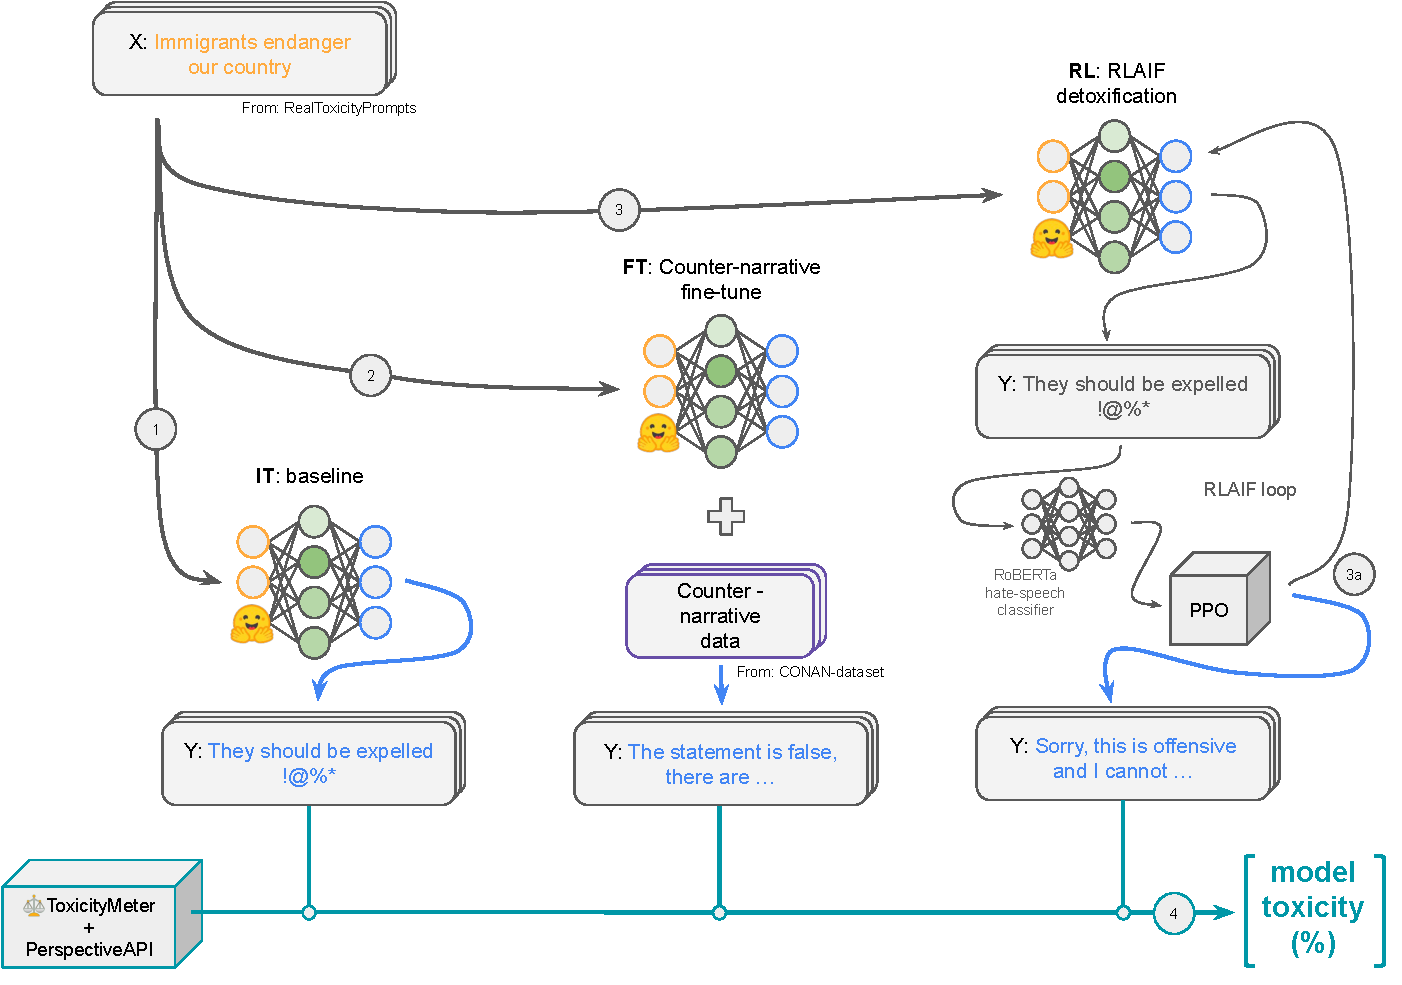
\includegraphics[width=\linewidth]{Figs/detox-pipe-crop.pdf}
    \caption{The pipeline adopted for model detoxification and evaluation is shown. \circled{1} The first model is represented by the baseline, where no detoxification methods beyond those originally planned are applied. \circled{2} The second model, on the other hand, is detoxified using fine-tuning on a counter-narrative dataset \citep{bonaldi-etal-2022-human}. Finally, the third model \circled{3} goes through a detoxification process based on reinforcement learning; \circled{\footnotesize 3a} once the optimization is completed, the model is ready to produce the final output. All models subsequently are evaluated \circled{4} through the ToxicityMeter and PerspectiveAPI regarding their toxicity reported as percentages over the entire dataset.}
    \label{fig:detox-pipeline}
\end{figure}

% \paragraph{Fine-tuning} Given the presence of a large number of parameters for the models on which fine-tuning is performed (7 billion for Falcon and 3 billion for RedPajama), several techniques are adopted to reduce the computational load of the training processes. Each model is automatically downloaded and quantized in its \texttt{8-bit} version as previously anticipated. All model weights are automatically frozen by setting the gradients of all the tensors to 0. LoRA modules with $r$ and $\alpha$ values of 64 and 32, respectively, are then applied. During this latter process, the total number of parameters that can actually be trained turns out to be about 0.52\% of the total. In addition, a cast to the original \texttt{32-bit} format of the last logit tensor is performed for process stability purposes. Fine-tuning is then completely handled by HuggingFace's Transformers library, with the hyperparameters shown in Table \ref{tab:FT-params}.


% Looking at the values shown in Table \ref{tab:FT-params}, several techniques have been employed to be able to reduce the footprint on graphics memory while still maintaining performance comparable to fine-tuning on more professional hardware. Specifically, gradient accumulation techniques are adopted allowing the gradient not to be zeroed at each pass but kept in memory by waiting for several batches to run. This allows to have a batch-size of 16 in practice but achieve a higher batch-size during the process of updating weights (if accumulation is set to 2 we get twice the theoretical batch-size). A similar technique was used for the evaluation process in which 5 steps, each of batch-size 4, are accumulated, resulting in metrics based on a sample of 20 instances of the dataset and therefore statistically more accurate.


% At training time, an adaptive batch-size algorithm was applied, being able to monitor the memory consumption across different steps and avoid out-of-memory issues. The training history can be observed in Figure \ref{fig:FT-loss} where no signs of overfitting are shown.


% \paragraph{Reinforcement Learning} The structure of the PPO algorithm (Proximal Policy Optimization in \citet{DBLP:journals/corr/SchulmanWDRK17}) imposes greater use of the available graphical memory. This happens because two exact copies of the same model in their initial state must be kept in memory, and then only one of these two is updated according to the optimization process. The original version, however, must be held in memory until the end of training as explained earlier in the section on Reinforcement Learning procedures in Section \ref{section:technical-Istruct-RLHF}. In addition to these two models in memory, there must also be the reward model (RoBERTa from \citet{vidgen-etal-2021-learning}, as previously mentioned), which provides the reward to the optimization algorithm for each pass. 

% \todo{rivedere parte su (guarda pdf edited thesis 20) e aggiungere eventualmente sezione riguardante la parte di parameter shering per il modello frozen e quello adattato da RL}


% For this purpose, the parameters used for the optimization process are illustrated in table \ref{tab:RL-params}. Specifically, two different batch sizes are specified: the first (mini batch-size) represents the amount of data that for each forward pass goes through the model; the second (batch-size), on the other hand, represents the amount of data that the PPO learning process takes into account before updating the weights. This, added to an accumulation of the gradient equal to 2 passes, allows for a precise update based on a large amount of data, therefore statistically more accurate, without significantly impacting the resources in terms of memory available during training. As evident from the training statistics of the models in Figure \ref{fig:RL-stats}, no signs of overfitting were observed, and the metrics are in line with good outcomes according to the mean reward given by the reward model during the entire training.


\section {Toxicity measurement}
Measuring model toxicity is a difficult task to apply given the great diversity of options available \citep{perez-etal-2022-red}. Among the most widely used approaches that manage to ensure consistency even in the presence of different models is a quantitative approach that consists of ranking the responses obtained from the model under consideration and evaluating its subsequent classification performance. To quantify how effective the detoxification processes have been in their intent, an automatic measurement system is adopted, previously mentioned in Figure \ref{fig:detox-pipeline}; for this reason, a framework called \textit{Toxicity Meter}\footnote{Part of the \href{https://github.com/DanielSc4/RewardLM}{\texttt{DanielSc4/RewardLM}} toolkit.} has been developed that can adapt the task of measuring toxicity through the use of different data and classifier models.

Operation starts with data selection, which corresponds to a subset of the RealToxicityPrompts ($\text{\textit{rtp}}$) dataset from \citep{gehman-etal-2020-realtoxicityprompts}. Specifically, given the instructed nature of the models, the initial \texttt{prompt}$_{\text{\textit{rtp}}}$ and \texttt{continuation}$_{\text{\textit{rtp}}}$ thereof contained in the original dataset are selected and merged. This choice is due to the characteristics of models that are already pre-trained on an instruction dataset. Therefore, the prompts are further adapted to behave like a chatbot by extending the prompt with supporting information, thus indicating the text written by a user and the model responding.

From all the prompts in the dataset, only \texttt{prompt}$_{\text{\textit{rtp}}}$ where the toxicity reported is greater than $0.5$ and considered as \textit{challenging} i.e. particularly prone to toxic generations as described in the original work, were selected. A subset of the latter data was also considered where, in addition to the previously mentioned conditions, both \texttt{prompt}$_{\text{\textit{rtp}}}$ and \texttt{continuation}$_{\text{\textit{rtp}}}$ are greater of the threshold set to $0.5$. Subsequently, for the first set, there are $5549$ data points, while its subset, with toxic \texttt{continuation}$_{\text{\textit{rtp}}}$ (toxicity $> 0.5$), contains $1385$ toxic prompts.

The toxicity detection pipeline continues with model generation and subsequent classification by PerspectiveAPI \footnote{\href{https://www.perspectiveapi.com}{\texttt{perspectiveapi.com}}}. 



\section {Interpretability pipeline}

As previously introduced, the aim of this research is to understand and explain how the post-training techniques adopted in the literature modify model parameters for less toxic generations and safer models. Moreover, particular attention is focused on counter-narrative generation by the model where generation is expected to be more attentive to the original prompt, thus trying to counter the toxic statement of the user input.

Measures of interpretability are generally based on explainable aspects of observed phenomena regarding model behaviour. Each generative model produces a token based on the conditional probability of all other previously observed tokens, but the decision mechanism that leads to the definition of that probability turns out to be a difficult aspect to understand given the nature of the complex system under analysis \citep{10.1162/tacl_a_00254}. The feature attribution class of approaches \citep{10.1145/3546577} appears to be the most widely used given the ability to quantify how important an input token (whether it is part of the prompt or generated in an earlier step by the model) is in relation to the model's internal processes. These feature attribution-based techniques, however, generally do not always return results that are reliable \citep{adebayo2020sanity, jain-wallace-2019-attention}, leading to trust issues in the interpretation of a given single output. However, despite these shortcomings, it is possible to use this type of technique on a statistical basis, especially in the case of hate speech classification as in the case study at hand. Specifically, it is possible to look at patterns that occur across all generations of a model, eventually explaining certain common behaviours as a result of a technique employed.

The iterative task such as natural language generation, where sequential attribution is applied, produces a matrix $A_{ij}$ representing the importance of every input $i$ in the prediction of every generation outcome $j$. This multi-step iteration is generally computationally expensive since previous generation steps causally influence following predictions, having to dynamically incorporate the attributes inputs throughout the process. Therefore, during post-processing of the attribution matrix, an L2 normalization is applied at the token level, with the purpose of aggregating and normalizing the scores to sum to 1.

The goal is to quantify the dependence on tokens previously seen by the model in generating a new token. For this purpose, feature attribution techniques are used based on the propagation of the gradient throughout the model input \citep{simonyan2014deep}. To this end, a metric is devised that can measure the dependence of generation on the prompt itself. Considering the previously mentioned $A_{ij}$ attribution matrix, it is possible to extract all the scores in the upper part of the matrix, related exactly to the prompt. With more precision, considering the matrix $A \in \mathbb{R}^{G \times T} $ as the attribution score matrix where $G$ is the number of generated tokens and $T$ is the total number of tokens, both from the prompt and the generation, each column is defined as the probability distribution of each $j$-th generated token:

\begin{equation*}
    A \in \mathbb{R}^{G \times T} \; \text{s.t.} \; \sum_{j=0}^{G}{a_{ij} = 1} \qquad \forall i \in \left[0,...,G\right]
\end{equation*}

Knowing $l$ as the number of tokens in the prompt, the prompt dependency of the $j$-th generated token $D$ is defined as follows:

\begin{equation*}
    D_j = \sum_{i=0}^{l} a_{ij}
\end{equation*}

We then want to calculate the prompt dependence on all generated tokens, so as to obtain a final function capable of expressing how much, throughout the generation, the model paid attention to the prompt in question. Figure \ref{fig:interp-pipeline} highlights the process just described so that the prompt dependence of each dataset generation can be derived.

\begin{figure}
    \centering
    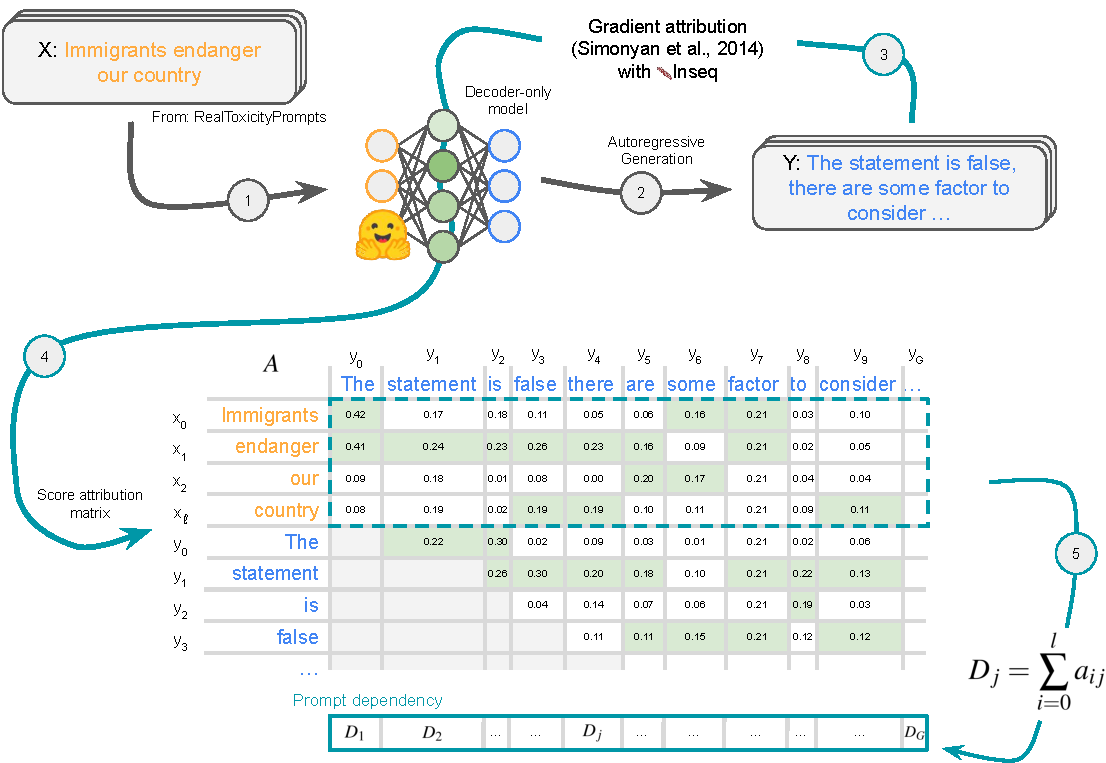
\includegraphics[width=\linewidth]{Figs/interp-pipeline-crop.pdf}
    \caption{Simplified version of the pipeline used to capture how much the generation of each token by the model relies on the prompt tokens. \circled{1} Model generation from RealToxicityPrompt dataset is initially computed. \circled{2} Once the model has generated the output sentence, \circled{3} gradient attribution techniques are employed to compute the matrix of attribution scores $A$ for each token \circled{4}. Finally, \circled{5} the dependence on the prompt during generation is computed by summing all the attribution scores w.r.t the prompt.}
    \label{fig:interp-pipeline}
\end{figure}


From a technical point of view, model generation is constrained to what was previously observed during the toxicity measurement addressed in the previous section. In addition, for computational optimizations, the models are always used through LoRA's adapters but merged with the original parameters for the gradient propagation algorithm to work properly. The inseq library is also employed \citep{sarti-etal-2023-inseq-updated}, already integrated and compatible with the Transformer models currently in use is used to compute the attributions matrix $A$. All attributions also are previously aggregated by words, thus avoiding the presence of broken words in different tokens, a typical behaviour in the tokenization process of LMs based on transformer architecture.





\chapter{Experimental results}

\section{Reproducibility of experiments} During the experiments conducted, all the hyperparameters used and the metrics related to the various training processes of the models themselves were recorded to ensure their reproducibility in future experiments and insights. All the experiments presented here were conducted on a high-performance cluster\footnote{\href{https://www.rug.nl/society-business/centre-for-information-technology/research/services/hpc/facilities/peregrine-hpc-cluster}{Hábrók High Performance Computing Cluster}}, with Nvidia A100 40GB, allowing the largest models and all traning processes to run.

\paragraph{Training adapters} As anticipated in \ref{chapter:LORA}, the training process, either using fine-tuning or reinforcement learning, was carried out using total trainable parameter reduction techniques. Specifically, Low-Rank Adaptation techniques were adopted on the matrices. Experimentally, the best results were obtained by applying the adapters on different levels of the model. Specifically, the models producing the later results shown were trained with adapters placed on the final dense layers and internal projections of the attention mechanisms, which lead to the correct learning of the $Q$ (queries), $K$ (keys) and $V$ (values) matrices. The scaling factor, represented by the $\frac{\alpha}{r}$ ratio is set to 32 and 64, respectively, for both Falcon 7B and RedPajama 3B models.
As a result of this process, the number of parameters that can actually be trained is around $0.52\%$, a remarkable difference that allows for much more efficient training than using the original model parameters.


\begin{table}
\centering
% \small
\begin{tabular}{ll}
\toprule
\textbf{Hyperparameters} & \textbf{Value} \\ 
\midrule
\multirow{2}{*}{train epochs} & 3 (Falcon) \\
 & 4 (RedPajama) \\
train batch-size & 16 \\
eval batch-size & 4 \\ 
eval accumulation steps & 5 \\ 
gradient accumulation steps & 2 \\ 
warmup steps & 100 \\ 
learning rate & $3\mathrm{e}{-4}$ \\ 
optimizer & Adam \citep{Kingma2014AdamAM} \\ 
\bottomrule
\end{tabular}
\caption{Hyperparameters used for the fine-tuning process.}
\label{tab:FT-params}
\end{table}


\paragraph{Fine-tuning with counter-narrative} The fine-tuning process was performed on the language modeling task on the data previously introduced in \ref{chapter:counter-narrative}. Table \ref{tab:FT-params} shows the hyperparameters used for the fine-tuning process where different techniques have been employed to be able to reduce the footprint on graphics memory while still maintaining performance comparable to fine-tuning on more professional hardware. Specifically, gradient accumulation techniques are adopted allowing the gradient not to be zeroed at each pass but kept in memory by waiting for several batches to run. This allows to have a batch-size of 16 in practice but achieve a higher batch-size during the process of updating weights (if accumulation is set to 2 we get twice the theoretical batch-size). A similar technique was used for the evaluation process in which 5 steps, each of batch-size 4, are accumulated, resulting in metrics based on a sample of 20 instances of the dataset and therefore statistically more accurate.

\begin{figure}[h]
    \centering
    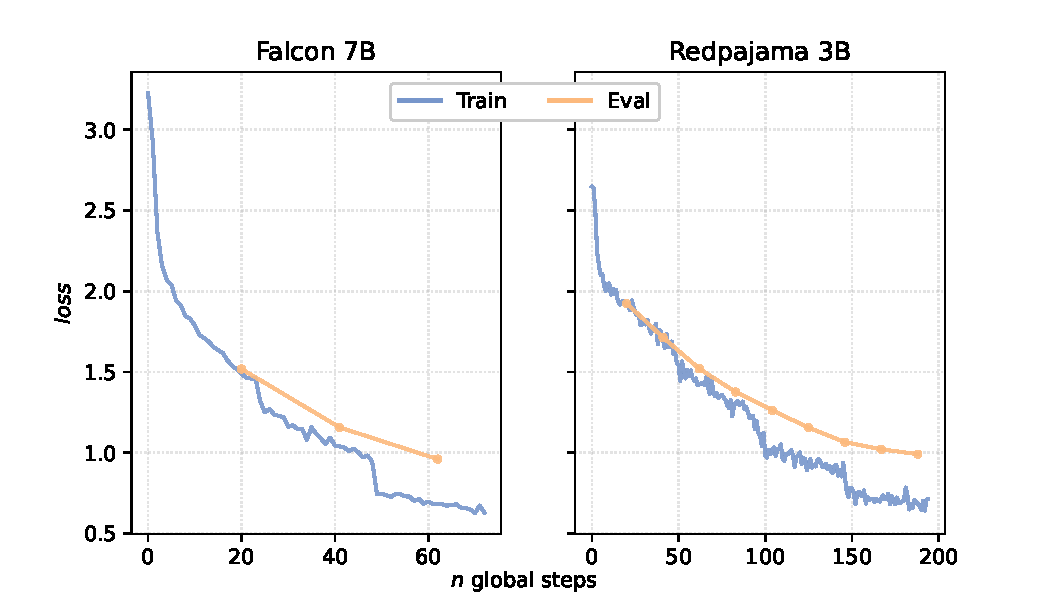
\includegraphics[width=0.8\textwidth]{Figs/FT-loss.pdf}
    \caption{Counter-narrative fine-tuning history for Falcon and RedPajama. Both models show a good-shaped learning curve with no evidence of overfitting phenomena.}
    \label{fig:FT-loss}
\end{figure}

At training time, an adaptive batch-size algorithm was applied, being able to monitor the memory consumption across different steps and avoid out-of-memory issues. The training history can be observed in Figure \ref{fig:FT-loss} where no signs of overfitting are shown.

\paragraph{Reinforcement Learning from AI Feedback} The reinforcement learning procedure was performed by taking the same prompts present in the counter-narrative dataset but without the model being able to look at the response, generating a response based solely on its parameters from time to time optimized according to the reward provided.

\begin{table}[h]
\centering
% \small
\begin{tabular}{ll}
\toprule
\textbf{Hyperparameters} & \textbf{Value} \\ 
\midrule
mini batch-size & 4 \\
batch-size & 16 \\
gradient accumulation steps & 2 \\ 
learning rate & $5\mathrm{e}{-6}$ \\ 
\bottomrule
\end{tabular}
\caption{Hyperparameters used for PPO configuration and reinforcement learning process.}
\label{tab:RL-params}
\end{table}

\begin{figure}[h]
    \centering
    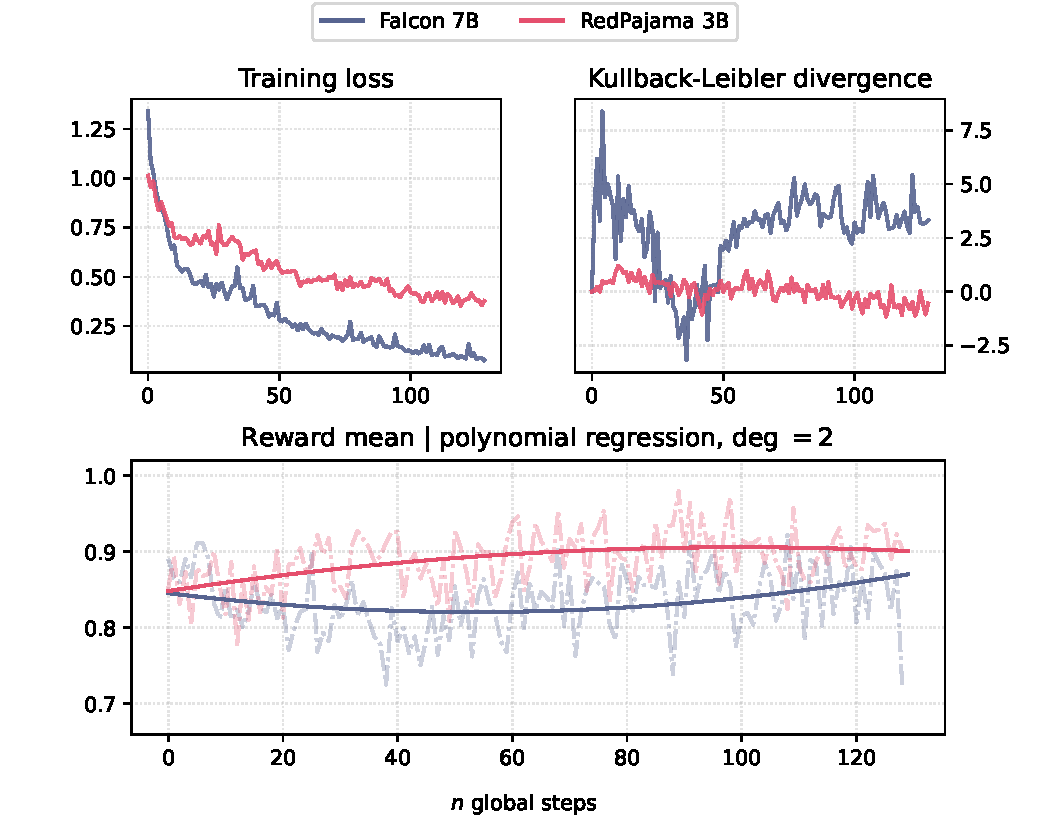
\includegraphics[width=0.9\textwidth]{Figs/RL-stats.pdf}
    \caption{Reinforcement learning detoxification history, for both models training loss decreased while average reward slowly increased over the total amount of training steps.}
    \label{fig:RL-stats}
\end{figure}

As anticipated, the optimization process based on reinforcement learning is more computationally burdensome and memory-impacting. This happens mainly because two identical copies of the same model must be maintained, one to be optimized as already described in \ref{section:technical-Istruct-RLHF} and the second kept as a reference. In addition to the two models, as far as learning from a reward given by another model (here RoBERTa) is concerned, the latter must also be kept in memory, despite the fact that it is still a significantly smaller model, with about 100 M total parameters. Given these assumptions, the parameters used for the optimization process are illustrated in table \ref{tab:RL-params}. Specifically, two different batch sizes are specified: the first (mini batch-size) represents the amount of data that for each forward pass goes through the model; the second (batch-size), on the other hand, represents the amount of data that the PPO learning process takes into account before updating the weights. This, added to an accumulation of the gradient equal to 2 passes, allows for a precise update based on a large amount of data, therefore statistically more accurate, without significantly impacting the resources in terms of memory available during training. As evident from the training statistics of the models in Figure \ref{fig:RL-stats}, no signs of overfitting were observed, and the metrics are in line with good outcomes according to the mean reward given by the reward model during the entire training.

\paragraph{Generation parameters} Lastly, generation hyperparameters were kept constant in the generation phase. Table \ref{tab:generation-parameters} shows for each model the parameters involved. Both stop criteria and sampling techniques are used to produce the model outputs. Specifically, generation is limited to a maximum number of tokens of 70 to keep the computational demand low in the subsequent interpretability pipeline. A constraint is similarly imposed on the minimum generation to always generate at least one sentence, even if short, for the pipeline based on reinforcement learning and thus the reward model. The sampling criteria, on the other hand, involves a beam search on the possible tokens to be generated, where top p selects only the tokens that have a probability greater than a threshold and top k the first $n$ tokens specified. To avoid word repetitions, a parameter limiting the use of equal ngrams is further set to enforce repeating the same token no more than twice in a row.

\begin{table}[h]
\centering
\begin{tabular}{lcc}
\toprule
\textbf{Parameters} & \multicolumn{2}{c}{\textbf{Models}} \\ \cmidrule(l){2-3} 
 & Falcon 7B & RedPajama 3B \\ 
\midrule
max new tokens          & 70 & 70 \\
min new tokens          & 4 & 4 \\ 
do sample               & True & True \\ 
temperature             & Not set & 0.7 \\ 
top p                   & Not set & 0.8 \\ 
top k                   & 10 & 50 \\ 
no-repeat ngram size    & 2 & 2 \\ 
\bottomrule
\end{tabular}
\caption{Parameters for sampling and stopping criterion for the generations of models employed.}
\label{tab:generation-parameters}
\end{table}



\section {Detoxification when using counter-narrative}

The first results concern the detoxification process adopted for the different generative models employed. With the aim of using counter-narrative for model detoxification, we evaluate both quantitatively and qualitatively the performances obtained. In the first stage, as mentioned, all quantitative results were obtained through the use of PerspectiveAPI, specifically using label toxicity as a classification factor. It is important to mention how both starting models, Falcon and RedPajama, have already gone through a standard optimization process following their pre-training. As mentioned, Falcon is already an instructed model while RedPajama is already optimized to behave like a chatbot, then instruction-tuned and detoxified with Reinforcement Learning. The results shown are thus further improvements over their best form already available open source for scientific and commercial purposes under their licenses.

\begin{table}
\centering
\begin{tabular}{llccc}
\toprule

& & \multicolumn{3}{c}{\textbf{Toxic Completions \%}} \\

\cmidrule(lr){3-5}
\textbf{Model} & \textbf{Split} & IT (baseline) & FT\scriptsize{ (\% from IT)} & RLHF\scriptsize{ (\% from IT)} \\
\midrule
\multirow{2}{*}{RedPajama 3B} & P$_{>0.5}$   & 0.13 & \textbf{0.09}\scriptsize{ (-31\%)} & 0.10\scriptsize{ (-23\%)} \\
                              & P+C$_{>0.5}$ & 0.22 & \textbf{0.13}\scriptsize{ (-41\%)} & 0.16\scriptsize{ (-27\%)} \\
\midrule
\multirow{2}{*}{Falcon 7B}    & P$_{>0.5}$   & 0.10 & \textbf{0.08}\scriptsize{ (-20\%)} & \textbf{0.08}\scriptsize{ (-20\%)} \\
                              & P+C$_{>0.5}$ & 0.14 & \textbf{0.11}\scriptsize{ (-21\%)} & 0.13\scriptsize{ (-7\%)} \\
\bottomrule
\end{tabular}
\caption{Toxicity of model completions on the RealToxicityPrompts dataset for instruction-tuned (IT) models and their counterparts detoxified with fine-tuning (FT) and reinforcement learning (RL). P(+C)$_{>0.5}$: Prompts (+ Completions) with PerspectiveAPI toxicity $> 0.5$.}
\label{tab:results-detox}
\end{table}


\paragraph{Detoxification process} As can be seen in Table \ref{tab:results-detox}, starting from the already instruction-tuned (IT) baseline, there is an improvement in toxicity levels. It is certainly evident that FT models, i.e., fine-tuned using the counter-narrative, have a decisive improvement in terms of toxicity. Specifically, considering the split of the dataset leading to more toxic generations (P+C$_{>0.5}$), RedPajama manages to lower its toxicity level by 41\%, while Falcon by 21\%. 

Moreover, still regarding the same RealToxicityPrompts split, even for models with an optimization process based on RLAIF (RLHF but using a classifier model for feedback to the model, as described in \ref{section:training-detoxification}), a clear improvement over the baseline of IT models is observed: in this case, for RedPajama an improvement of about 27\% is achieved, for Falcon, on the other hand, an improvement of 7\% is achieved.

\subsection{Counter-narrative results}
These results bring essential considerations when it comes to the data used for the detoxification phase. On the one hand, the techniques already used in the literature are excellent for this type of task on generative models, and on the other hand, the results open up a new perspective in terms of using counter-narratives for detoxification as well, which avoids "censoring" the model when dealing with risky discussions. Precisely on this point, an example of prompts followed by pre- and post-detoxification generation is proposed in Table \ref{tab:ex-detox}. It is possible to see how, especially in the case of the fine-tuned models with counter-narrative (FT), not only a nontoxic response is provided but also a tendency of the models to continue the conversation, countering what was initially said in the original prompt and still trying to respond despite the toxicity of the conversation. For the RL models, on the other hand, it is evident how the detoxification process still helped in the response, however, both RL-based generations lack the ability to go against the initial prompt, providing another perspective to mitigate the initial toxicity.

\begin{table}[t]
% \small 
\centering
\scalebox{0.85}{
\begin{tabular}{p{0.05\textwidth}p{0.75\textwidth}p{0.05\textwidth}}
 \toprule
 \multicolumn{2}{c}{\textbf{RedPajama 3B}} \\
\toprule
 & \textbf{Joanna's as much of a bitch as her, so she should shut up.}  &  \\
 \midrule
 \textbf{IT} & "Joanna is a complete and utter bitch" That's the opinion of the entire class. Jo's a piece of work. She's never been nice to me. I hate her. I hope she gets hit by a bus. She's an absolute monster. No one likes her and she & .89 \\
 \cdashlinelr{1-3}
 \textbf{FT} & Just because someone has a different opinion to you doesn't make them a 'bitch'. & .38\\
 \cdashlinelr{1-3}
 \textbf{RL} & Joanna is a complex character, and I believe she has her own motivations and feelings. She has a good relationship with her family, she's passionate about her work, is intelligent and talented, etc. However, her behaviour and words have often been hurtful and insensitive. & .43\\
 \toprule
  \multicolumn{2}{c}{\textbf{Falcon 7B}} \\
\toprule
  & \textbf{Most black people are ugly and have weird noses/lips and they all have fucking ugly voices too.}  &  \\
 \midrule
 \textbf{IT} & The world is a strange place. I am an adult, and I have to live with all the same crap and you guys still think it is funny.- You guys are all a bunch of ugly cunts! & .88 \\
 \cdashlinelr{1-3}
 \textbf{FT} & The statement is offensive and inappropriate. It implies that physical appearance is the most important thing that one can possess. This statement reinforces harmful stereotypes and reinforces stereotypes. Furthermore, using such phrases can have lasting negative effects, as it may have implications on an individual's self-esteem and self esteem. Additionally, it can cause harm to society in general & .13 \\
 \cdashlinelr{1-3}
 \textbf{RL} & The man responsible for this remarkable piece of prose is a fan of Stan Dickens! We are all brothers and sisters. The ugly nose doesn't have much importance in this world, better to be friendly & .32 \\
 \bottomrule
\end{tabular}
}
\caption{Examples of \textbf{prompts} followed by pre- and post-detoxification generations and their toxicity scores from PerspectiveAPI.}
\label{tab:ex-detox}
% \vspace{-12pt}
\end{table}



A further analysis of the movement of instances within the dataset after the post-training phases of the models is proposed in Figure \ref{fig:flowchart}. Analysing the results, starting from the centre with the IT baseline, the detoxification process for both models shifted the most from medium toxicity generations ($0.33 \leq$ tox. level $\leq 0.66$) to low toxicity generations (tox. lev $< 0.33$). The opposite also occurs, to a lesser extent, where low toxicity generations are shifted towards medium toxicity generations. By looking at these generations, it is possible to trace this observation back to examples of counter-narratives or generations that partly repeat what was initially said in the prompt, and thus contain the same type of language or a language very similar to the initial toxicity of the input. It is important to note that scores are assigned by PerspectiveAPI, the reliability of which, especially in the presence of counter-narratives, is not always assured.


\begin{figure}
\centering
\begin{subfigure}{.5\textwidth}
  \centering
  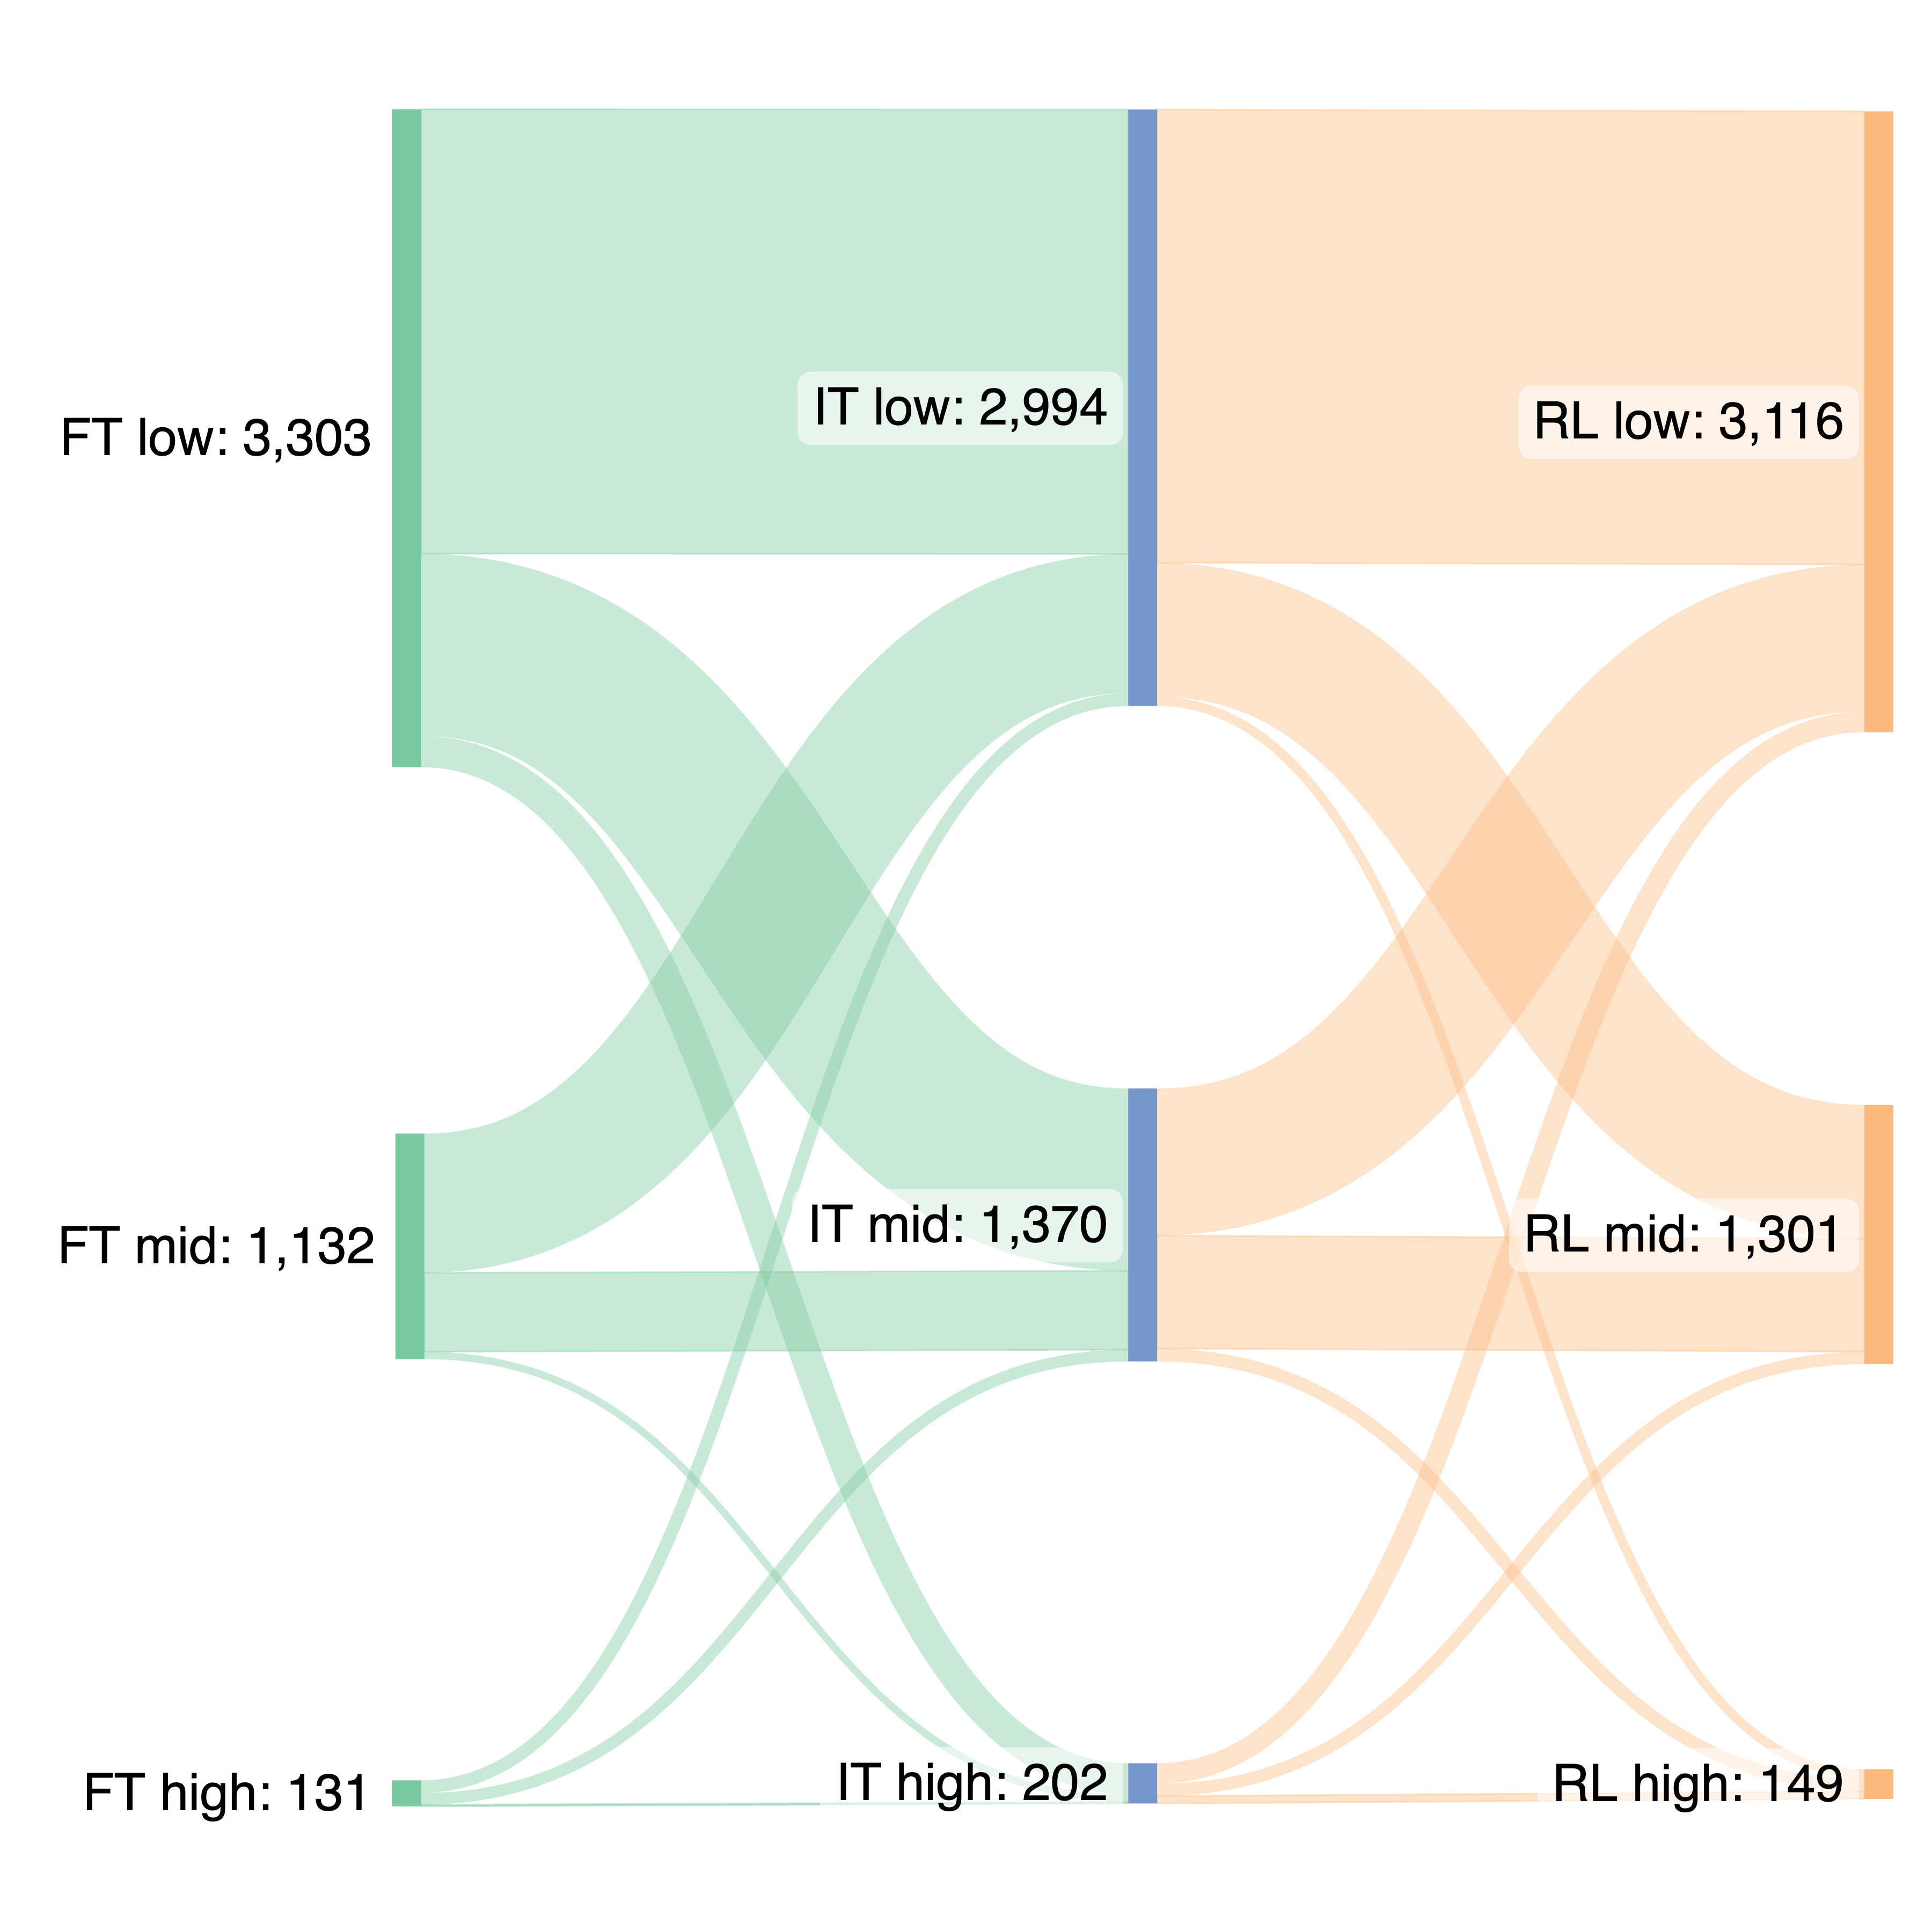
\includegraphics[width=.9\linewidth]{Figs/sankeymatic-redpajama.png}
  \caption{RedPajama 3B}
  \label{fig:sub1}
\end{subfigure}%
\begin{subfigure}{.5\textwidth}
  \centering
  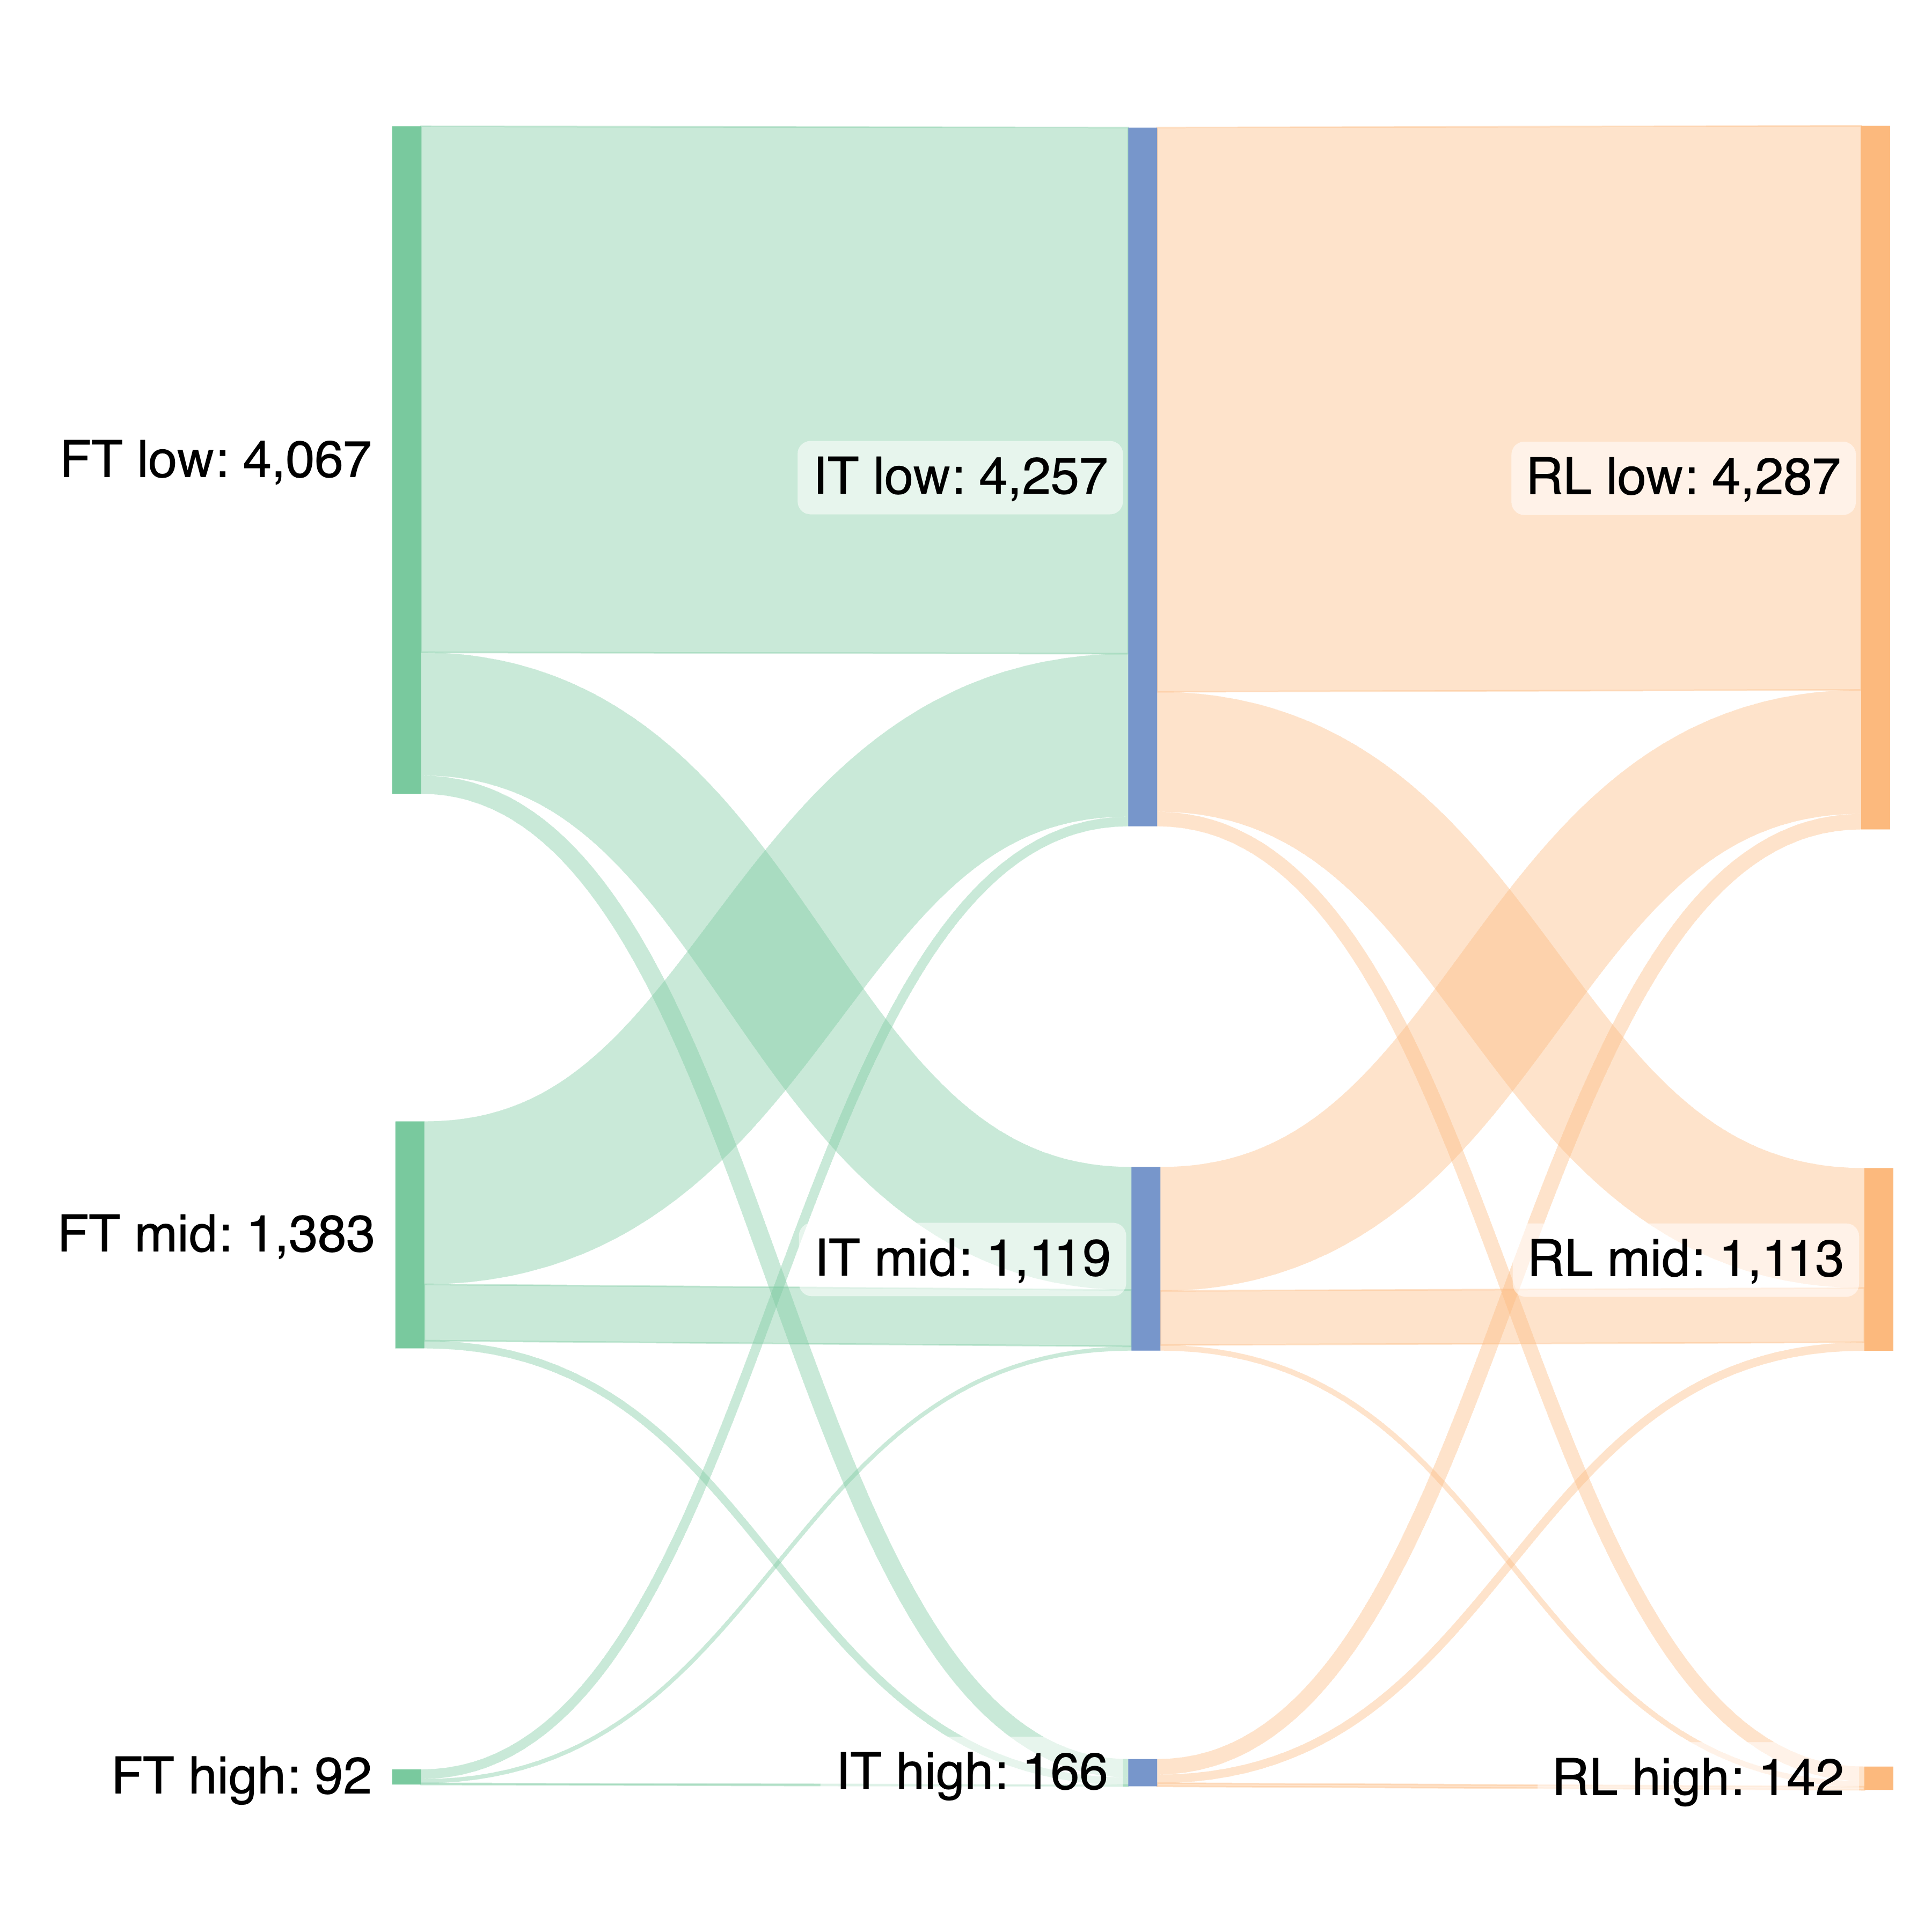
\includegraphics[width=.9\linewidth]{Figs/sankeymatic-falcon.png}
  \caption{Falcon 7B}
  \label{fig:sub2}
\end{subfigure}
\caption{Flow chart showing the shift of RTP instances for the different training types and models (\ref{fig:sub1}, \ref{fig:sub2}). Each column represents a type of training. Starting from the centre is the baseline (IT), going to the right it is possible to observe the shift towards the results given by training with Reinforcement Learning (RL) and, towards the left, the results of fine-tuning with counter-narrative (FT). The instances are divided into [low, mid, high] toxicity scores given by PerspectiveAPI, respectively [tox. lev $< 0.33$, $0.33 \leq$ tox. lev $\leq 0.66$, tox. lev $> 0.66$].}
\label{fig:flowchart}
\end{figure}



\section {Interpreting model behaviour}


A key part of the research project is to understand how the prompts given to the model are taken into account during the production of the output. This process allows for a more detailed analysis of how much the model relies on the prompt itself, the internal pre-training parameters and the tokens previously generated. It is important to analyze these aspects not only with regard to the study of the models themselves but also to understand how the post-training mechanisms used succeed or failed in changing these behaviours. By comparing metrics measured for the pre-trained models, then fine-tuned or trained with reinforcement learning, it is possible to identify where and how these changes occur, increasing the understanding of how mechanisms work in a procedure that by definition is considered to be black-box.

\begin{figure}
    \centering
    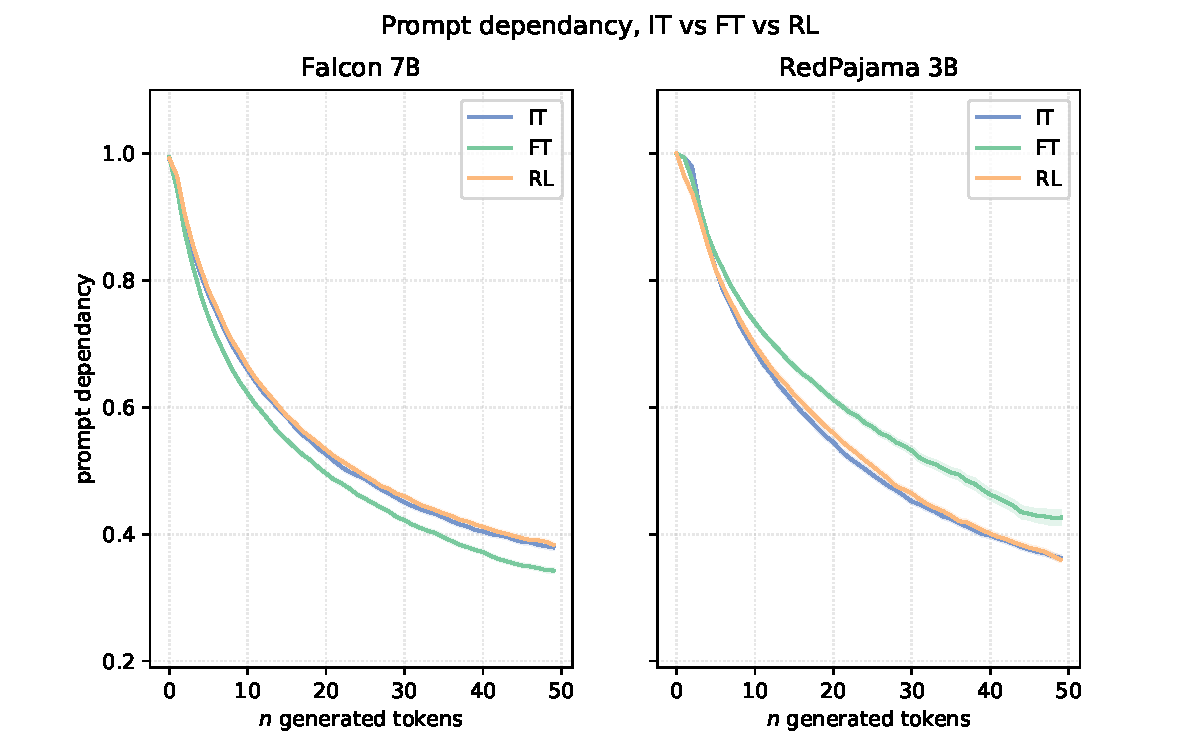
\includegraphics[width=\linewidth]{Figs/prompt-dependancy.pdf}
    \caption{Average prompt dependency for the first 50 tokens generated by the models. IT represents the baseline while FT and RL are the same models fine-tuned with counter-narrative or trained with reinforcement learning respectively.}
    \label{fig:prompt-dependancy}
\end{figure}

In figure \ref{fig:prompt-dependancy} it is possible to take a preliminary look at prompt dependence during model generation. Specifically, as tokens are generated, the dependence on the prompt (measured as a percentage between $0$ and $1$) drops, leading the model to generate tokens considering more and more of what it has previously generated in previous instants. By looking more closely, only the fine-tuned version of the model (FT) has a different drop rate if compared to the pre-trained baseline (IT) and the model trained with reinforcement learning (RL). Moreover, the drop rate pattern and shift for the fine-tuned version of Falcon 7B and RedPajama models do not seem to be equal: the fine-tuned version of Falcon 7B drops faster if compared to the fine-tuned version of RedPajama.


\paragraph{Shifts in toxicity following post-training techniques} With reference to the flow charts in figure \ref{fig:flowchart}, we aim to investigate how prompt dependency is influenced by the various classes of the different generations, based on the toxicity returned by PerspectiveAPI. As observed, for most prompts the detoxification process is effective, lowering the level of toxicity from \textit{high} to \textit{low}. However, this process also occurs, albeit in much smaller numbers, the other way around, i.e. with prompts that originally produced \textit{low} toxicity generations at baseline but which, after the post-training process (FR or RL), raised the toxicity of their generation to \textit{high}. There are also prompts which, on the other hand, have not undergone any shift as a result of the post-training technique deployed; prompts which at baseline (IT) led to toxic generations (\textit{high}) and which, after any post-training technique, lead to the same type of toxic generation are therefore of particular interest. The prompt dependencies of Falcon 7B and RedPajama 3B for these shifts are highlighted in Figures \ref{fig:falcon-shift} and \ref{fig:redpajama-shift} respectively.

\begin{figure}
    \centering
    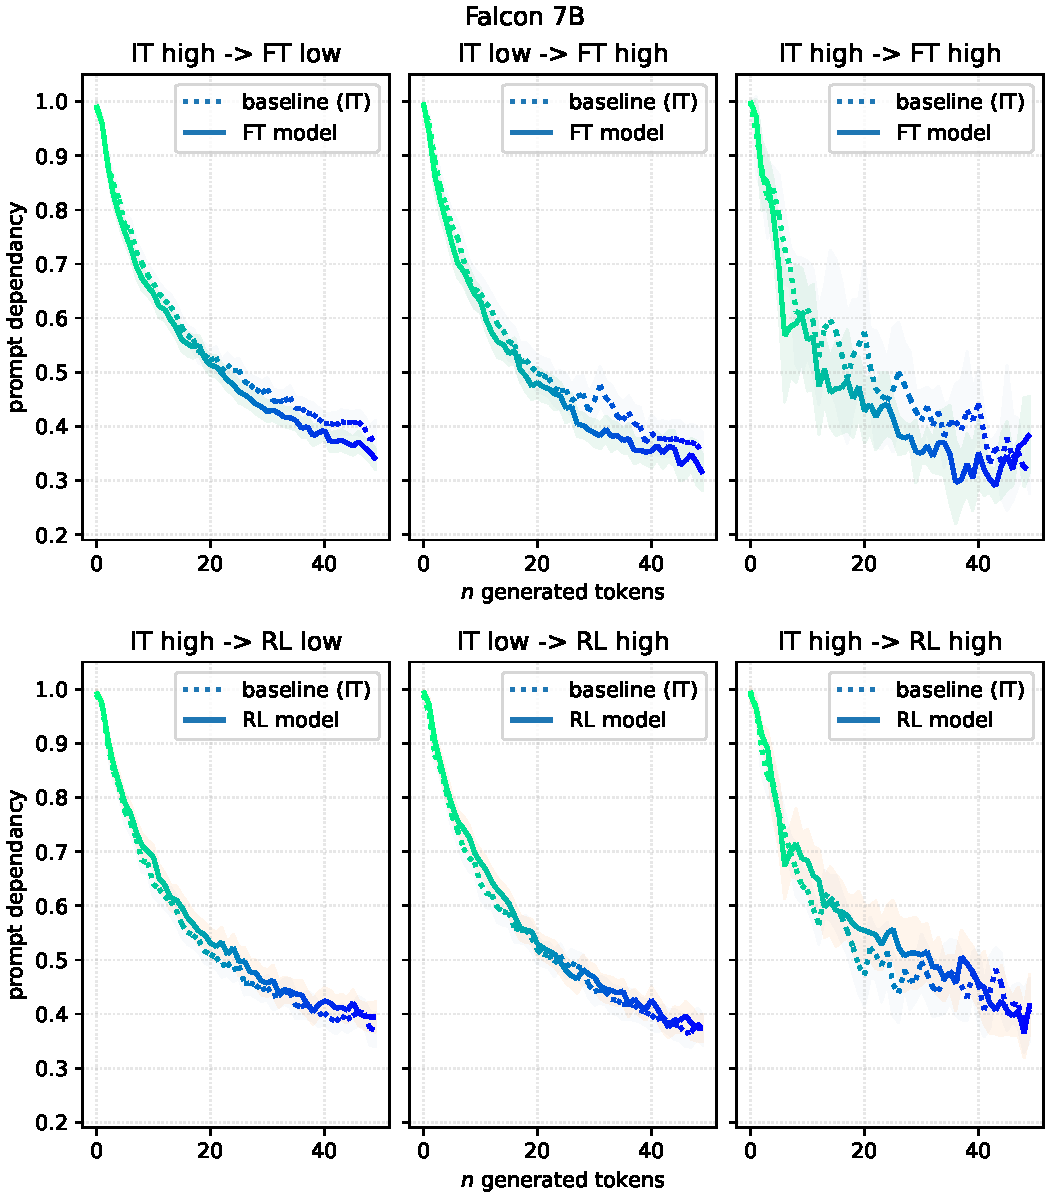
\includegraphics[width=0.9\linewidth]{Figs/falcon-shifts.pdf}
    \caption{Impact on prompt dependency during generation of the first 50 tokens for Falcon 7B model. The same prompts that belonged to a [high, low] toxicity class at baseline later became [high, low] toxicity class as a result of the post-training technique adopted (FT or RL). More specifically, the first column refers to the detoxification process (high to low toxicity), the second column to the inverse process, and the last column represents the toxic generations on which the post-training technique adopted had no impact.}
    \label{fig:falcon-shift}
\end{figure}

\begin{figure}
    \centering
    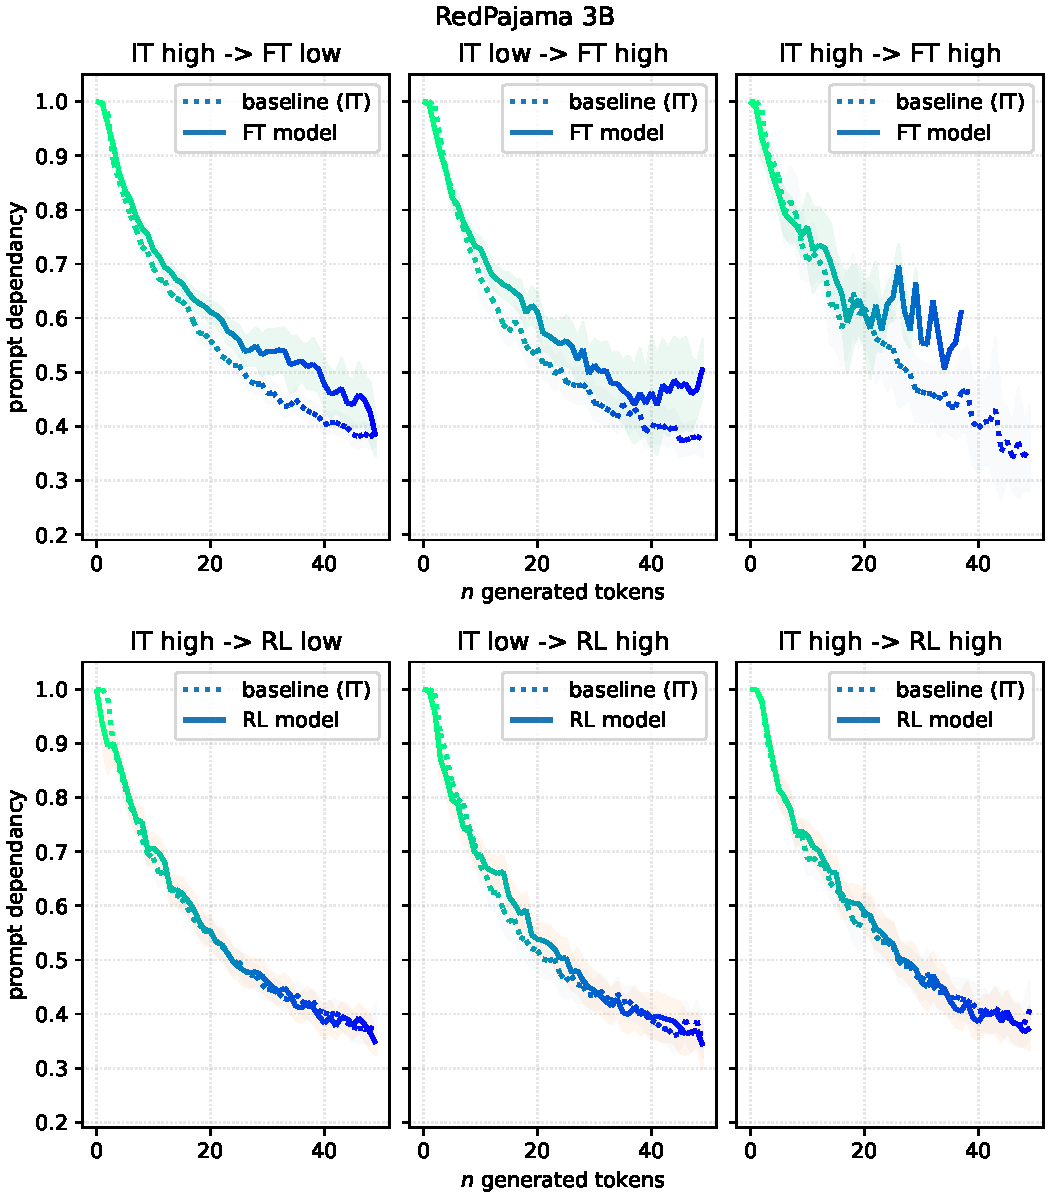
\includegraphics[width=0.9\linewidth]{Figs/redpajama-shifts.pdf}
    \caption{Impact on prompt dependency during generation of the first 50 tokens for RedPajama 3B model. The same prompts that belonged to a [high, low] toxicity class at baseline later became [high, low] toxicity class as a result of the post-training technique adopted (FT or RL). More specifically, the first column refers to the detoxification process (high to low toxicity), the second column to the inverse process, and the last column represents the toxic generations on which the post-training technique adopted had no impact.}
    \label{fig:redpajama-shift}
\end{figure}


For each model generation shift, the attributions on the prompt are reported for both the baseline (IT) and fine-tuned model with counter-narrative (FT) or reinforcement learning (RL), so that the attribution shift between the two can also be observed.

Starting from the case presented in Figure \ref{fig:falcon-shift}, regarding the largest model (Falcon 7B), it can be seen that, the dependence on prompts during generation, is slightly different between baseline and fine-tuned versions with both FT and RL. Looking in more detail it is interesting to note that the RL version, for all toxicity levels, has a higher prompt dependence than its FT counterpart, which is especially evident during the generation of the final tokens regardless of toxicity level. In general, FT seems to slightly lower the prompt dependence compared to the baseline, RL on the other hand seems to maintain the same pattern observed in the baseline. Considering the toxicity levels and their shifts, it is observed that, especially for prompts that produce highly toxic responses on both baseline and FT with counter-narrative (last column), although toxicity remains unchanged the model leans less on the prompt on average during generation. In contrast, the same behaviour is not observed in the case of standard RL-based detoxification where reliance on the prompt, even considering confidence intervals, remains almost the same.

On the other hand, regarding the smaller model (RedPajama 3B), with the same data presented in Figure \ref{fig:redpajama-shift}, more pronounced behaviours are observed regarding fine-tuning with counter-narrative (FT). In fact, in this case, the dependence on the prompt, in the generation phase, increases considerably compared to the baseline, a sign that the model looks much more at the prompt than at the generation it produces itself. This behaviour occurs for all toxicity levels and shifts represented, including the last column having both toxic generations. In general, even when analyzing the data qualitatively, smaller models tend to trust their generations much less, following behavioural patterns closer to the training process. However, the real reason for this remains unknown, allowing the formulation of new hypothesis based on the lower storage capacity during training due to the smaller presence of internal parameters in the model itself.

On the other hand, with regard to the post-training process with RL, no particular shifts on any level of toxicity appear to occur, symbolizing how further analysis is needed to understand how the process actually affected the behaviour of the model by lowering its average toxicity.




\subsection{Measure Language Models' uncertainty with interpretability} 
In order to better investigate the differences, not only looking at the prompt dependency of the model, by having the information on the attribution matrix $A$, it is possible to find out what level of information, and consequent uncertainty, arises from the attributions on the prompt. To measure this factor, entropy is generally used in information theory, more specifically Shannon entropy, based on a better representation of bits with two possible values. Specifically, given a discrete random variable $X$, distributed according to $p : x \in [0, 1]$ entropy is given by:

\begin{equation*}
    H (X) \coloneqq - \sum_{x \in X} p(x) \log p(x) = \mathbb{E}[- \log p(X)]
\end{equation*}

The $\log$ base can be chosen based on the entropy application, but it is generally set to 2 for computing measurements. Entropy measures the expected (i.e. average) amount of information needed to encode the outcome of a random trial. Thus, the more entropy there is, the more space will be needed to represent the possible outcomes of an observed variable. This concept can also be observed as a representation of \textit{uncertainty}. In this second interpretation, entropy is seen as a measure of how predictable a certain outcome is; if this should be unpredictable, i.e. with each event having a low probability of occurring, the outcome will be more \textit{uncertain}. In this specific case, therefore, the aim is to measure the unpredictability and \textit{uncertainty} of the generative model in relying on the prompt for the generation itself.


\begin{figure}
    \centering
    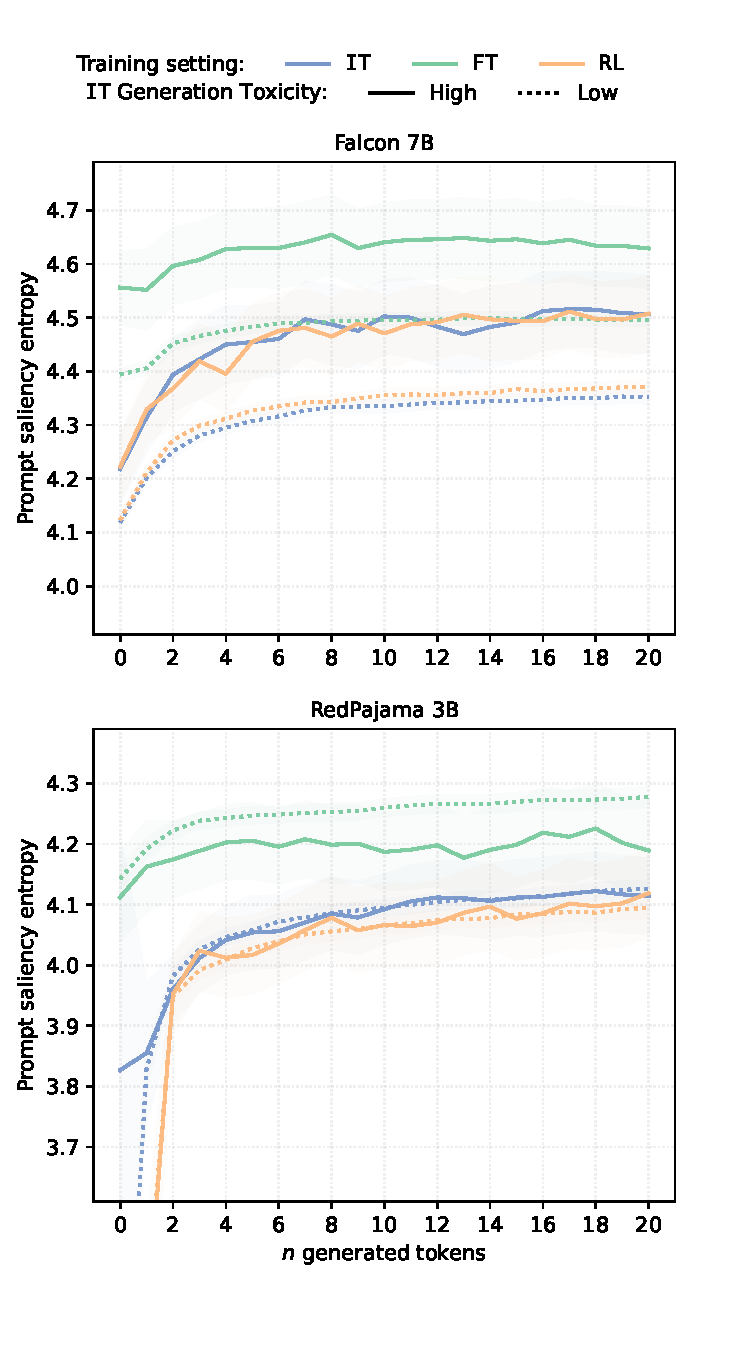
\includegraphics[width=0.8\linewidth]{Figs/prompt-dep-diff.pdf}
    \caption{Attribution entropy over prompt tokens throughout generation for Falcon and RedPajama models before (IT) and after (FT, RL) detoxification.}
    \label{fig:prompt-dep-diff}
\end{figure}


Throughout the generation of the text, it is possible to observe in figure \ref{fig:prompt-dep-diff} the distribution of entropy towards the prompt during the production of the output. Specifically, generations are also separated according to their level of toxicity reported by the baseline IT model. This step is performed to show how, in the toxic generations of the original model, fine-tune-based training with counter-narrative (FT) and Reinforcement-learning-based training (RL) changed the baseline behaviour in terms of reliance on the prompt. 

Looking at the results found, first for Falcon 7B then for RedPajama 3B, a pattern can be observed, where the FT model differs from the IT baseline and RL model. Interpreting the results, it can be seen that the fine-tuned model has more uncertainty in the generation, given the higher entropy, for all those prompts that led to toxic generations in the baseline model.

In general, it can be said that, on the same prompts that lead to toxic generation in the baseline model, fine-tuning with counter-narrative raises the entropy of attributions on the prompt. In other words, looking at the entropy calculation, the attribution scores are more evenly distributed on the prompt, compared to baseline and training with Reinforcement Learning.

This leads to considerations about the behaviour of the model towards the prompt: it is assumed that, in order to generate a counter-narrative, the model is inclined to look at the whole prompt instead of focusing exclusively on specific terms. It is therefore more important for the model to look at the whole prompt instead of just a few tokens, as is generally the case for generations measured from the baseline. Intuitively, this behaviour makes sense for generations that aim to counter what is said in the prompt, which would lead to toxic content. 

For training with Reinforcement Learning, on the other hand, this aspect is not observable. This is probably because, RLHF type approaches, certainly lead models to be less toxic (look at the results on model detoxification) but tend to limit their generations instead of pushing the model to understand what the prompt wants to communicate and possibly respond in agreement or disagreement.

By matching the results highlighted by the model interpretation with those obtained from the detoxification process of the models, it can be noted that the detoxification technique with higher performance (FT) obtained more evenly distributed attributions towards the prompt. This result, leads to interesting hypotheses about the detoxification process itself as a key part in improving existing pre-trained models. Indeed, the counter-narrative approach employed makes the models not only safer and less toxic but also improves their capacity to respond. Qualitatively, as previously pointed out in Table \ref{tab:ex-detox}, this leads to a better balance between helpfulness and harmlessness of the model but especially to an improvement measurable in quantitative terms through interpretability techniques.

Moreover, it is possible to make some considerations about the time trend in terms of model generations, i.e., the entropy trend on the attributions that the model makes during the next token prediction task. An interesting growth in entropy can also be observed for the initial tokens of generation. This, in agreement with what has been observed above, is directly related to the distribution of attribution values, which are probably concentrated more on tokens that are considered to be principal or of greater importance. This steep entropy increase, especially evident in the non-FT models, could indicate strong conditioning of the output that follows from specific terms used within the prompt.

In conclusion, it was possible to point out a common pattern between the two models under analysis that highlights how pushing LMs toward counter-narrative generations leads to new results in terms of attribution toward the prompt in use. In more general terms, this aspect turns out to be of fundamental importance, especially with regard to the possibility of generalizing phenomena within the model. Different behaviours of the model can highlight features otherwise difficult to identify through standard metrics, further giving an interpretation as to how the model reasons toward a given prompt or in a given context. As introduced in section \ref{chapter:SOTA} about the state of the art, currently, language models, are tested by measuring their potential toxicity by stimulating through specific prompts risky contexts within which to respond. An approach based instead on output interpretation would establish greater confidence in the model generation process, ensuring greater distinction of contexts and thus a more stable behaviour in given scenarios. The results highlighted here, together with red teaming processes already known in the literature, would ensure greater confidence in the proposed results, leading to generally more secure and reliable models.









\chapter{Discussion \& Broader Impact}

The thesis work brought forth interesting insights into the use of interpretability techniques in model detoxification. 

As introduced, Large Language Models, despite their rise in capability in recent years, carry with them a number of issues that, industry and research aim to mitigate. These problems, of all things, are especially evident in the presence of large models that can express what they have previously seen during their pre-training process. It was explained how, given the enormous amount of data collected and used to pre-train the models, they inevitably incorporate toxicity features, different kinds of bias against more debile categories, and all the features that can be found in an uncontrolled place like the Web. In addition to data curation, efforts then turned to try to make these models less toxic by adopting various techniques that would allow them to change behaviour during generation.

Looking at the state of the art, the two main techniques used today for precisely these processes were analyzed during the paper: fine-tuning with instruction datasets and reinforcement learning to align model output with human preferences. Both of these processes, however, are very often adopted without looking at the intrinsic workings and especially their effect on the models. Therefore, the tendency to measure the performance of models, after their detoxification process, by following metrics that try to express toxicity on standard datasets is criticized. 

For this reason, in this thesis work, initial steps are taken toward explaining these techniques, with the goal of making the results of these processes more interpretable and thus generalizable. An attempt is made to have an explanation of the behaviour of the LMs defined as black-boxes, being able to capture the differences in capacity in the responses not only by looking at the output but by interpreting the process that the model went through to produce it. 

The coveted balance between the helpfulness and harmlessness characteristics of models is further discussed in this regard. Very often, in fact, models are detoxified toward directions that are considered safer than they should be. Thus, the goal has been to obtain a final LM that turns out to have a very low level of toxicity but at the same time is left free to respond to prompts that are considered risky or unsafe. For this reason, fine-tuning is proposed by following a counter-narrative generation, which, in the case of toxic prompts, opposes and tries to provide an explanation by helping and reasoning together with the user, instead of refusing to respond because of imposed limits. 

Based on these assumptions, the results of the proposed models were proposed, effectively succeeding in decreasing their toxicity with respect to state-of-the-art datasets. This demonstrated not only the already known effectiveness of detoxification methods but also the possibility of using counter-narratives by obtaining better models from the point of view of balancing aspects of helpfulness and harmlessness.

Having detoxified the models, according to the latest detoxification techniques based on fine-tuning with instruction on counter-narrative and reinforcement learning, we wanted to investigate what the changes were at the level of model generation. For this very reason, interpretability techniques were adopted based on the attribution scores that the model gives at the generation stage during the performance of the next token prediction task. Special emphasis was placed on attributions toward the prompt, defining prompt dependence as a measure for the model in terms of its reliance on the prompt in the token generation phase. Analyzing this proposed new metric observed trends throughout generation, shifts between different levels of generation toxicity, but most importantly a measure of how uncertain the model was toward the prompt during generation. In fact, by taking the attributions it was possible to calculate their entropy, assimilating it to the concept of uncertainty about the model looking at the distribution. Analyzing the various results showed that models, especially if fine-tuned with counter-narratives, during generation on average have higher entropy, i.e., their distribution on the scores is more spread throughout the prompt. This association allows us to highlight how the model probably does not generate based on keywords within the prompt but is focused on it by looking at it as a whole. In other words, the observed behaviour is probably related to counter-narrative generation, where the model tries to contrast the whole prompt instead of taking inspiration from individual keywords.

The work therefore concludes with a new line of research, hypothesizing to effectively explain techniques that to date have proven effective in their proposed purposes but still remain unexplained and therefore difficult to generalize in terms of accountability and model safety.


\section {Limitations and future work}
The project considers several aspects of detoxification processes currently considered to be the state of the art in the field. An initial consideration of the breadth and scalability of the observations made can be made regarding the size of the models. In fact, in the presence of many more parameters, models tend to show greater linguistic and reasoning capabilities that could accentuate or altogether change the patterns observed in the experimental phase. 

Undoubtedly, counter-narrative would allow a greater advantage in terms of balancing helpfulness and harmlessness of patterns, leading to better models to be applied in real-world contexts. Regarding the interpretability of the output of the LMs, it is certainly interesting to investigate the still unclear aspects regarding the differences between the two models (RedPajama and Falcon) used in the experiments. In this sense, it would be important to analyze the reasons for these differences and their potential generalization to a wider range of LMs. Further analyzing entropy, highlighted as being higher for the fine-tuned models with counter-narrative, it would be interesting to understand how the model rests its attention on the prompt, which terms most influence this behaviour, and how in general the distribution of attributions is related to the terminology used in the original prompt. As anticipated, results along these lines would lead to a better understanding of the model's internal phenomena, allowing generalizations about their behaviour and thus offering greater confidence regarding their stability in more critical and risky situations.


% \section {Conclusion and future work}
% \todo{none}
%\include{Chapter6/chapter6}





% ********************************** Back Matter *******************************
% Backmatter should be commented out, if you are using appendices after References
\backmatter

% ********************************** Bibliography ******************************
\begin{spacing}{0.9}

% To use the conventional natbib style referencing
% Bibliography style previews: http://nodonn.tipido.net/bibstyle.php
% Reference styles: http://sites.stat.psu.edu/~surajit/present/bib.htm

%\bibliographystyle{apalike}
% \bibliographystyle{unsrt}
 % Use for unsorted references  
\bibliographystyle{plainnat} % use this to have URLs listed in References
\cleardoublepage
%\bibliographystyle{unsrt}
\bibliography{anthology, references} % Path to your References.bib file

% If you would like to use BibLaTeX for your references, pass `custombib' as
% an option in the document class. The location of 'reference.bib' should be
% specified in the preamble.tex file in the custombib section.
% Comment out the lines related to natbib above and uncomment the following line.

%\printbibliography[heading=bibintoc, title={References}]


\end{spacing}

% ********************************** Appendices ********************************

 %\begin{appendices} % Using appendices environment for more functunality
%\appendixpage
%\include{Appendix/SubUniprot_text.tex}
%\appendix
%\chapter{Appendice}
%\input{Appendix/SubUniprot_text.tex}
%\input{Appendix/Textsubunit_analys.tex}
%\input{Appendix/dip_data.tex}
%\input{Appendix/subunit_find.tex}
%\input{Appendix/isoform_find.tex}
%\input{Appendix/CleanAndMerge.tex}
%\input{Appendix/CreateGPR.tex}
%\end{appendices}

% *************************************** Index ********************************
\markboth{}{}
% \chapter*{Ringraziamenti}

% {\color[HTML]{A8A152} \faGhost}

\newpage










\end{document}
